\documentclass[ExampleMasters.tex]{subfiles}
%\usepackage{amsmath}
%\usepackage{graphicx}
%\usepackage[margin=1.3in]{geometry}
%\usepackage{float}
%\usepackage{caption}
%\usepackage{subcaption}


\begin{document}

%\centerline{\sc \large Long combinations with additional electric propulsion}
%\vspace{.5pc}
%\centerline{\sc Model validation results}
%\centerline{Karthik Venkataraman, 880128-T539}

%\listoffigures

\chapter{Model Validation}

\section{Introduction}
This document presents the findings from the analysis of the longitudinal modeling of the long vehicle combination structure with additional electric propulsion on specific axles. The design variables, or model parameters, in this analysis include the following:

\begin{itemize} 
\item Gross Combination Weight (GCW)
\item Axle loads on propelled axles
\item Engine size
\item Electric Machine sizing / rating
\item Electric buffer capacity and operating range
\item Buffer State of Charge (SoC) management
\end{itemize}

The influence of each of the above model parameters on the vehicle operating parameters and performance coefficients is analysed to serve as an adequate model validation. Reasonable trends in the output parameters will yield confidence in the physical modelling of the long vehicle combination and qualify the model to be used in optimising the axle propulsion configuration using a genetic algorithm.\\

Broadly listed, the output signals / parameters are as follows:

\begin{itemize}
\item Mission time
\item Fuel consumption
\item Charge consumption patterns over the mission and total charge consumed
\item Combination startability
\item Minimum combination speed at high gradients (alternatively, combination gradeability at specific speeds)
\item Mission productivity
\item Percentage of the mission that is power limited in operation nature
\item Percentage of the mission that is traction / grip limited in operation nature
\end{itemize}

\section{Vehicle model and simulation}

In all cases, the long combination considered is the standard A-Double, consisting of a 6X4 tractor (Unit 1), 3-axle semitrailer (Unit 2), 2-axle dolly (Unit 3) and another 3-axle semitrailer (Unit 4), in order. Specific combinations were chosen to demonstrate the influence of the model parameters on the outputs and these results are documented in this report. The A-Double propulsion configurations used for analysis were the following:

\begin{itemize}
\item Pure Combustion combination - 011-000-00-000
\item One axle on the first semitrailer propelled - 011-010-00-000
\item One axle each on the first semitrailer and dolly  propelled - 011-010-01-000
\item One axle each on all three trailing units propelled - 011-010-01-010
\item All axles on all three trailing units propelled - 011-111-11-111
\end{itemize}

The GCWs considered are 50t, 60t, 70t and 80t. The axle/unit loading in each case is listed in Table \ref{table:unitLoads}.\\

\begin{table}[ht]
\caption{Individual unit loads} 
\centering 
\begin{tabular}{c c c c c}
\hline\hline    
Unit number & GCW=50t & GCW=60t  & GCW=70t & GCW=80t \\
 \hline
    1  & 18080 & 18420 & 22434 & 22434\\
    2  & 15100 & 20100 & 22100  & 22400\\
    3  & 7000 & 8000 & 10500 & 12500  \\
    4  & 10000 & 13480 & 13480 & 22400 \\
\hline 
\end{tabular}
\label{table:unitLoads} 
\end{table}

The axle propulsion configuration of a specific combination is represented as in the below example. 
Combination 011-010-00-001 indicates:
\begin{itemize}
\item Axle 1 dead, Axles 2 and 3 propelled in Unit 1
\item Axle 1 and 3 dead, Axle 2 propelled in Unit 2
\item Both Axles 1 and 2 dead in Unit 3
\item Axles 1 and 2 dead, Axle 3 propelled in Unit 4
\end{itemize}

The mission selected for validation and optimisation is G\"oteborg-Malm\"o, spanning a distance of approximately 294 km. The gradient profile of the route is shown in Figure \ref{roadGradient}.

\begin{figure}[h!]
\centering
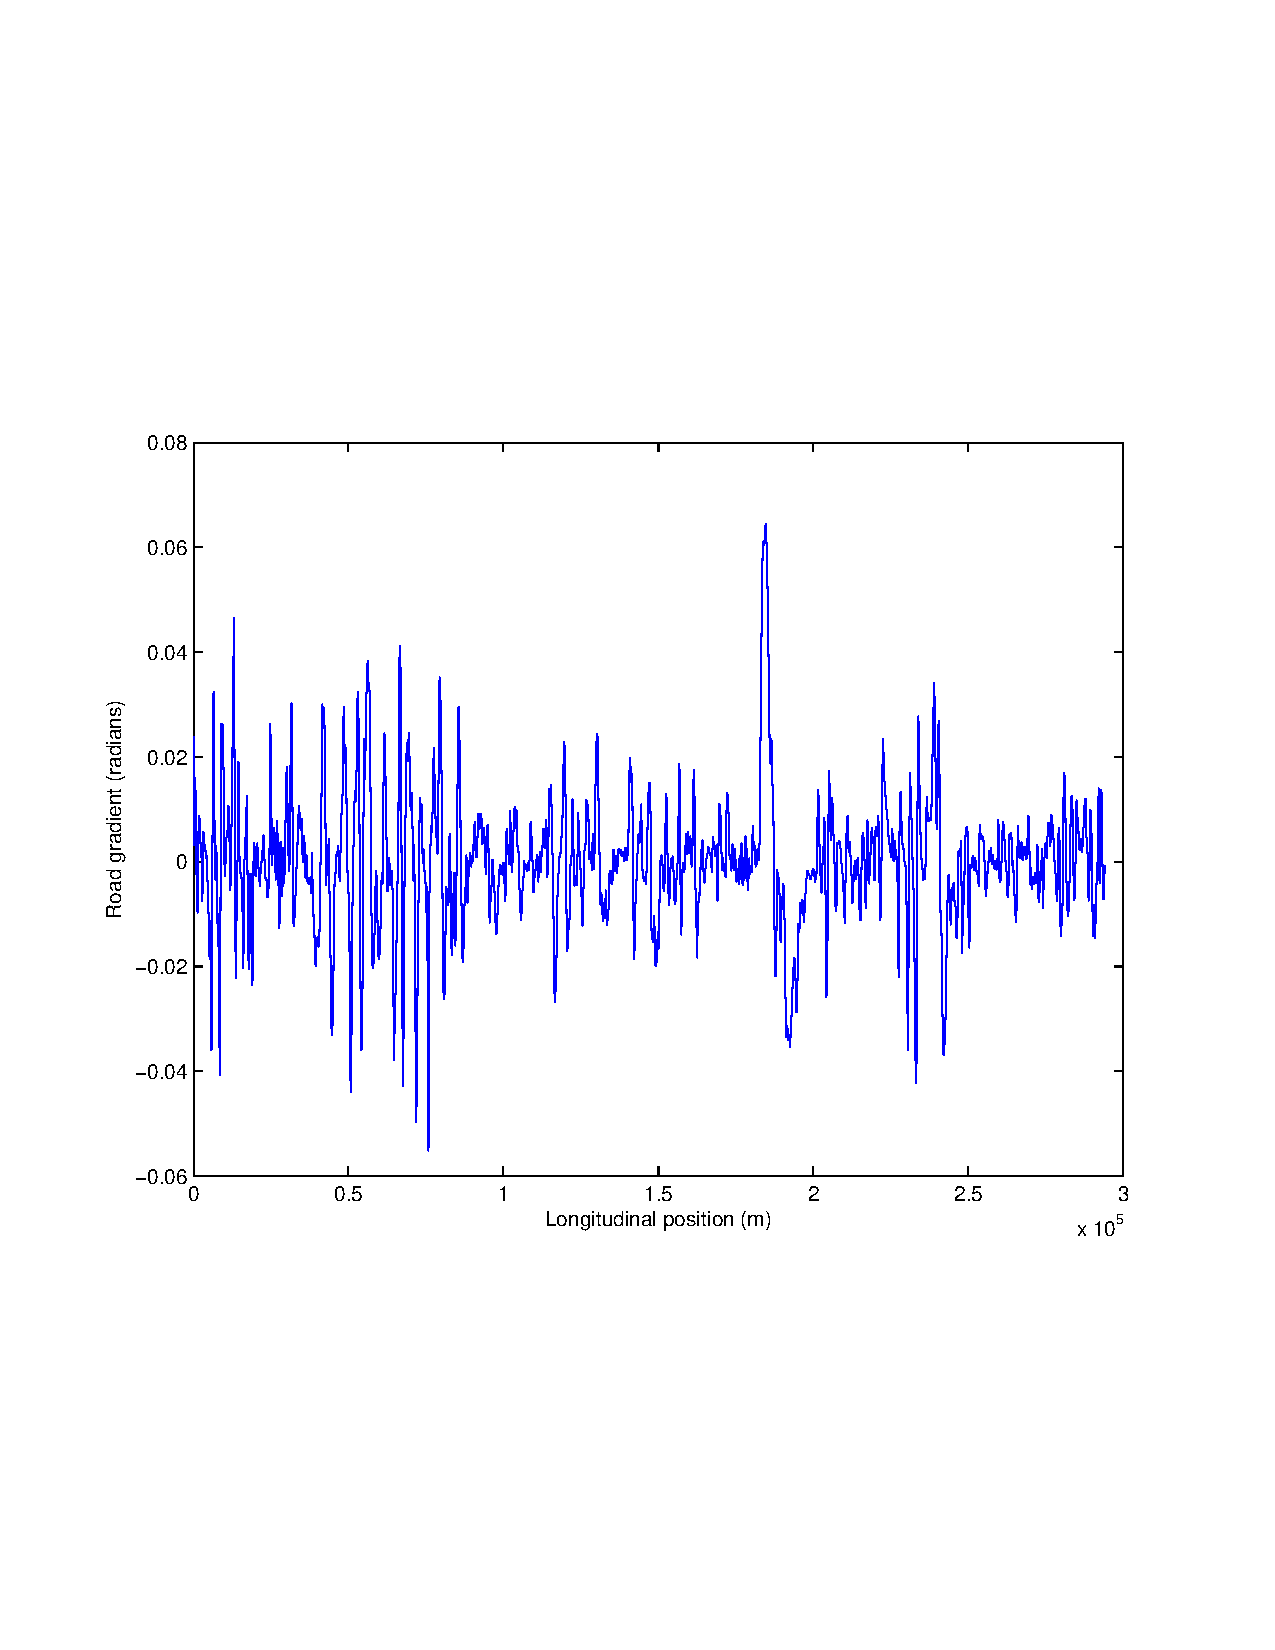
\includegraphics[width=80mm, clip=true, trim=45 185 65 208]{figures/ModelValidation/roadGradient.pdf}
\caption{Road gradient vs longitudinal position}
\label{roadGradient}
\end{figure}

The engines used for simulating the tractive machine in the tractor are the D11K450 EU6, D13C540 EU5 and D16G750 EU5 Volvo engines. The electric motors used are of ratings 120kW \& 230Nm, 173kW \& 411Nm and  180kW \& 420Nm. The electric buffers used on each unit are of capacities 4976640, 6272640 and 5987500 Coulombs.\\

The simulation whose results are dealt with below involved a constant target speed of 80kmph throughout the mission. Also, individual buffers were assigned constant depths of discharge in this preliminary exercise.

\section{Results and discussion}
Results are presented in subsections, each pertaining to a specific model parameter's role in the vehicle performance. For example, the effect of increasing gross combination weight keeping the axle propulsion configuration and engine size constant is discussed in a single subsection. All variations and ramifications of the single parameter in this context shall be covered in the same section.

\subsection{Engine Size and GCW}
The combination propelled \textit{solely by the tractor combustion engine} was tested first to observe the effects of the engine size and gross combination weight on the mission performance. As expected, for a given engine, mission time and fuel consumption increases with increasing GCW as shown in Figure \ref{timeFuelGCWEngine}. Increasing the GCW from 50t to 80t showed a 39\% increase in fuel consumption for the D11 and D13 engine powered combinations and a 36\% increase in fuel consumption for the D16 engine powered combination. The percentage increase in mission times for the D11, D13 and D16 engine powered combinations was 2.56\%, 1.71\% and 1.36\% respectively.\\

\begin{figure}[h!]
\begin{subfigure}{.5\textwidth}
	\centering
	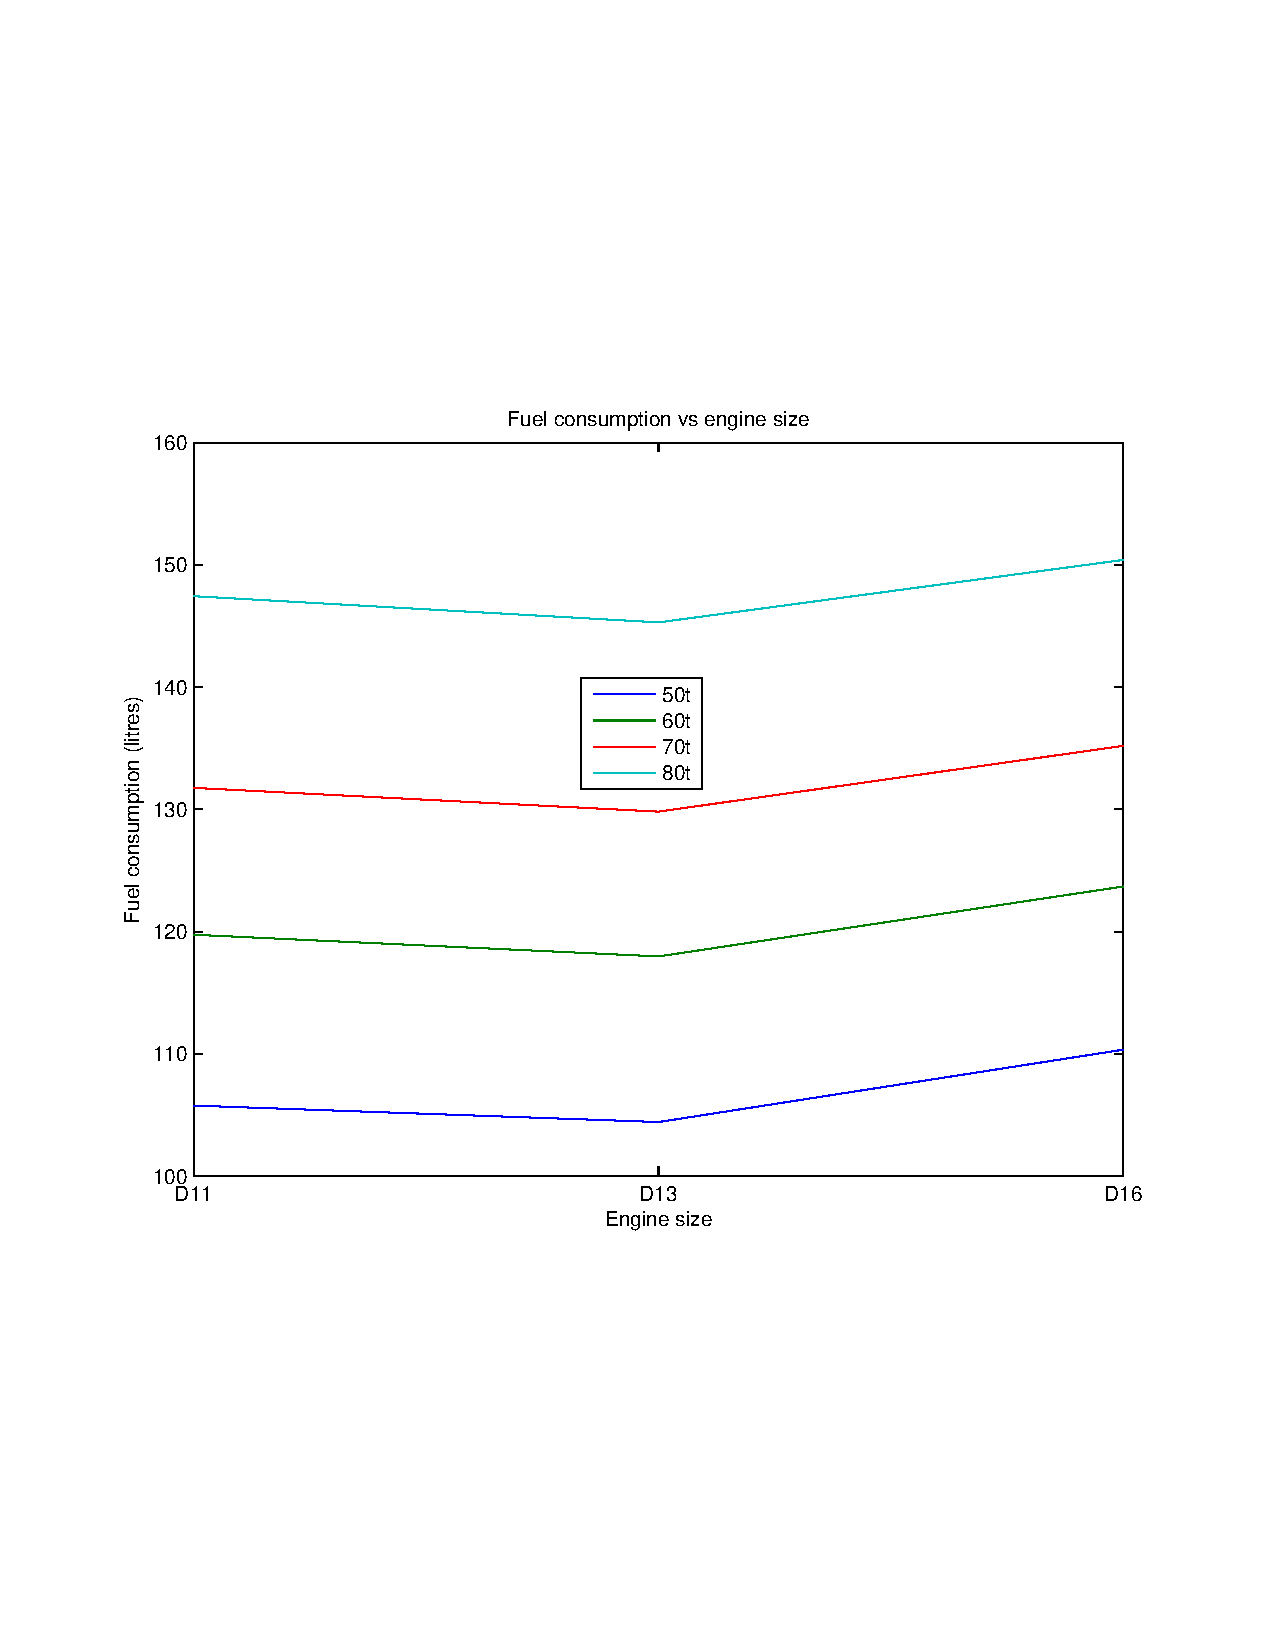
\includegraphics[width=\linewidth, clip=true, trim=45 185 65 208]{figures/ModelValidation/Engine_size_and_GCW/Fuel_consumption_vs_GCW_and_engine_size.pdf}
	\caption{Fuel consumption over mission}
\end{subfigure}
\begin{subfigure}{.5\textwidth}
	\centering
	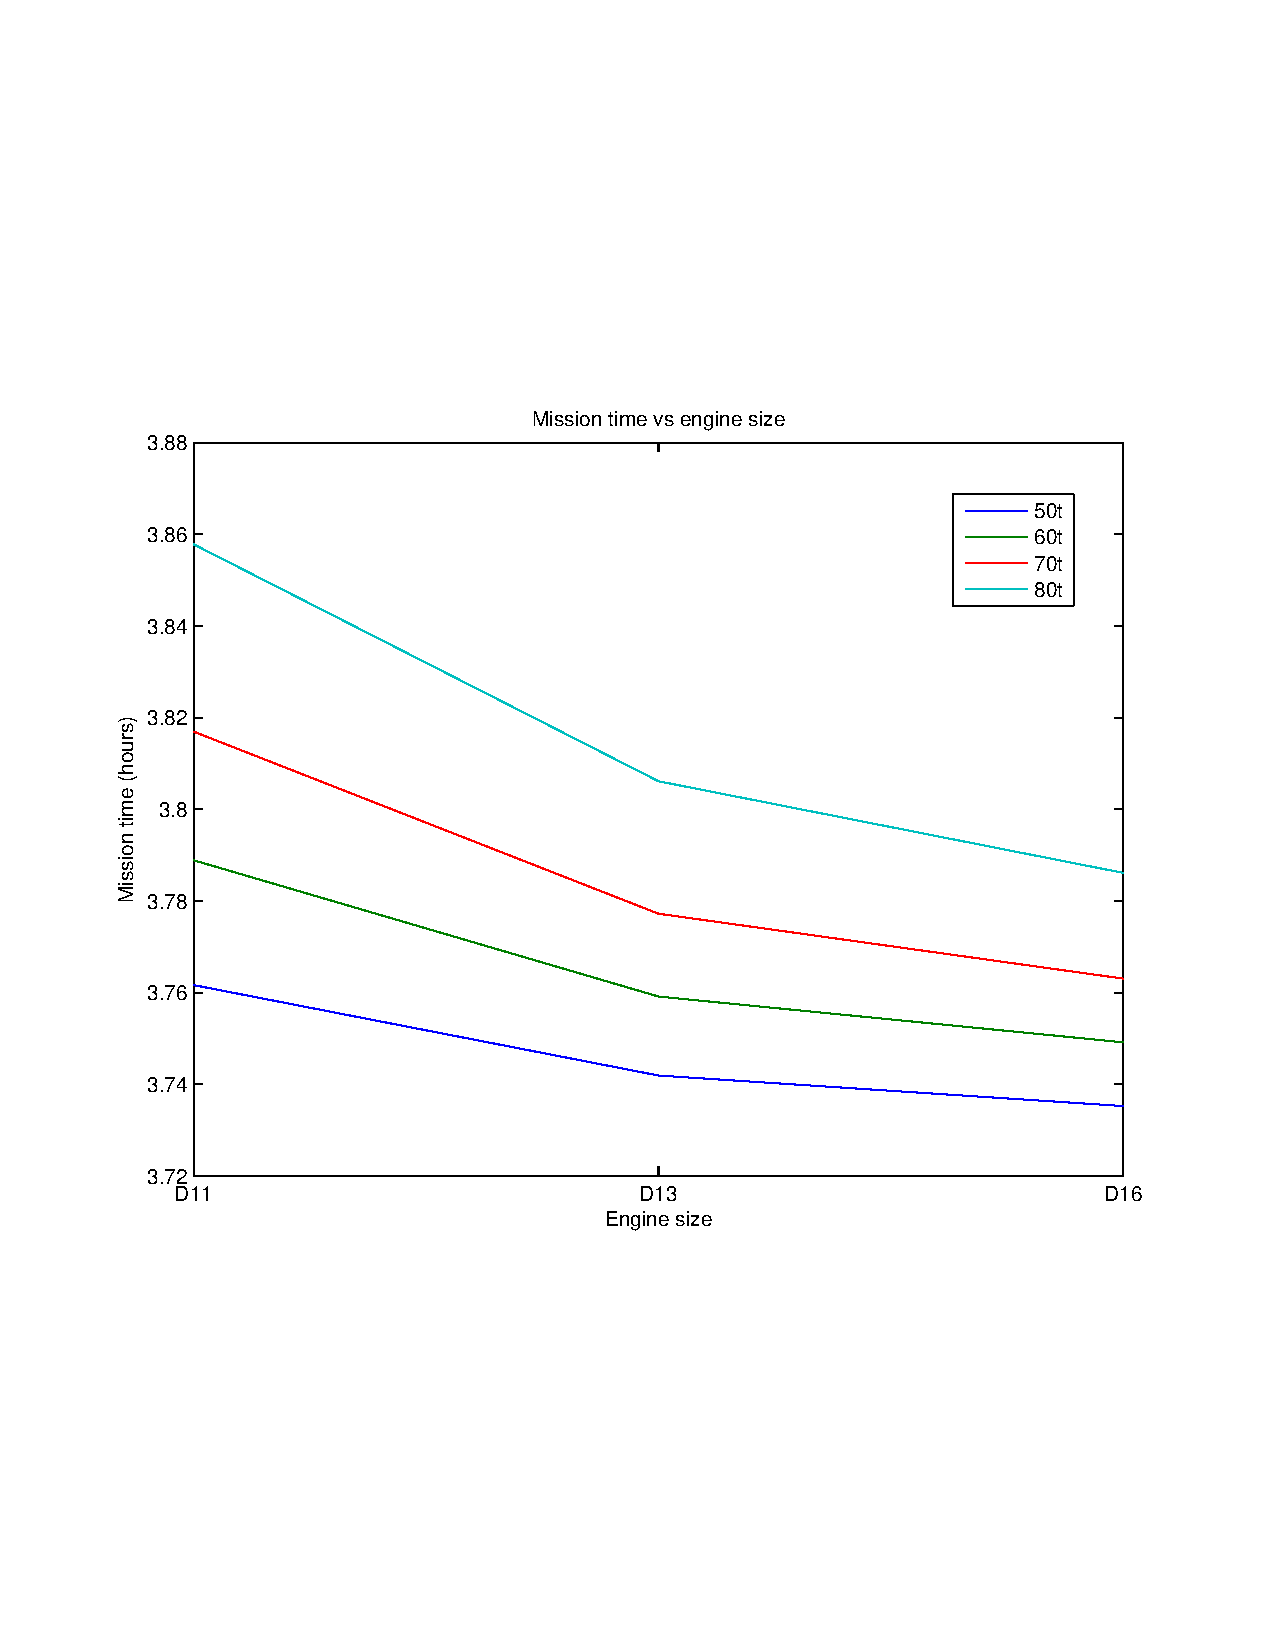
\includegraphics[width=\linewidth, clip=true, trim=45 185 65 210]{figures/ModelValidation/Engine_size_and_GCW/Mission_time_vs_GCW_and_engine_size.pdf}
	\caption{Mission time}
\end{subfigure}
\caption{Effect of engine size and GCW on fuel consumption and mission time}
\label{timeFuelGCWEngine}
\end{figure}

\begin{figure}[h!]
\centering
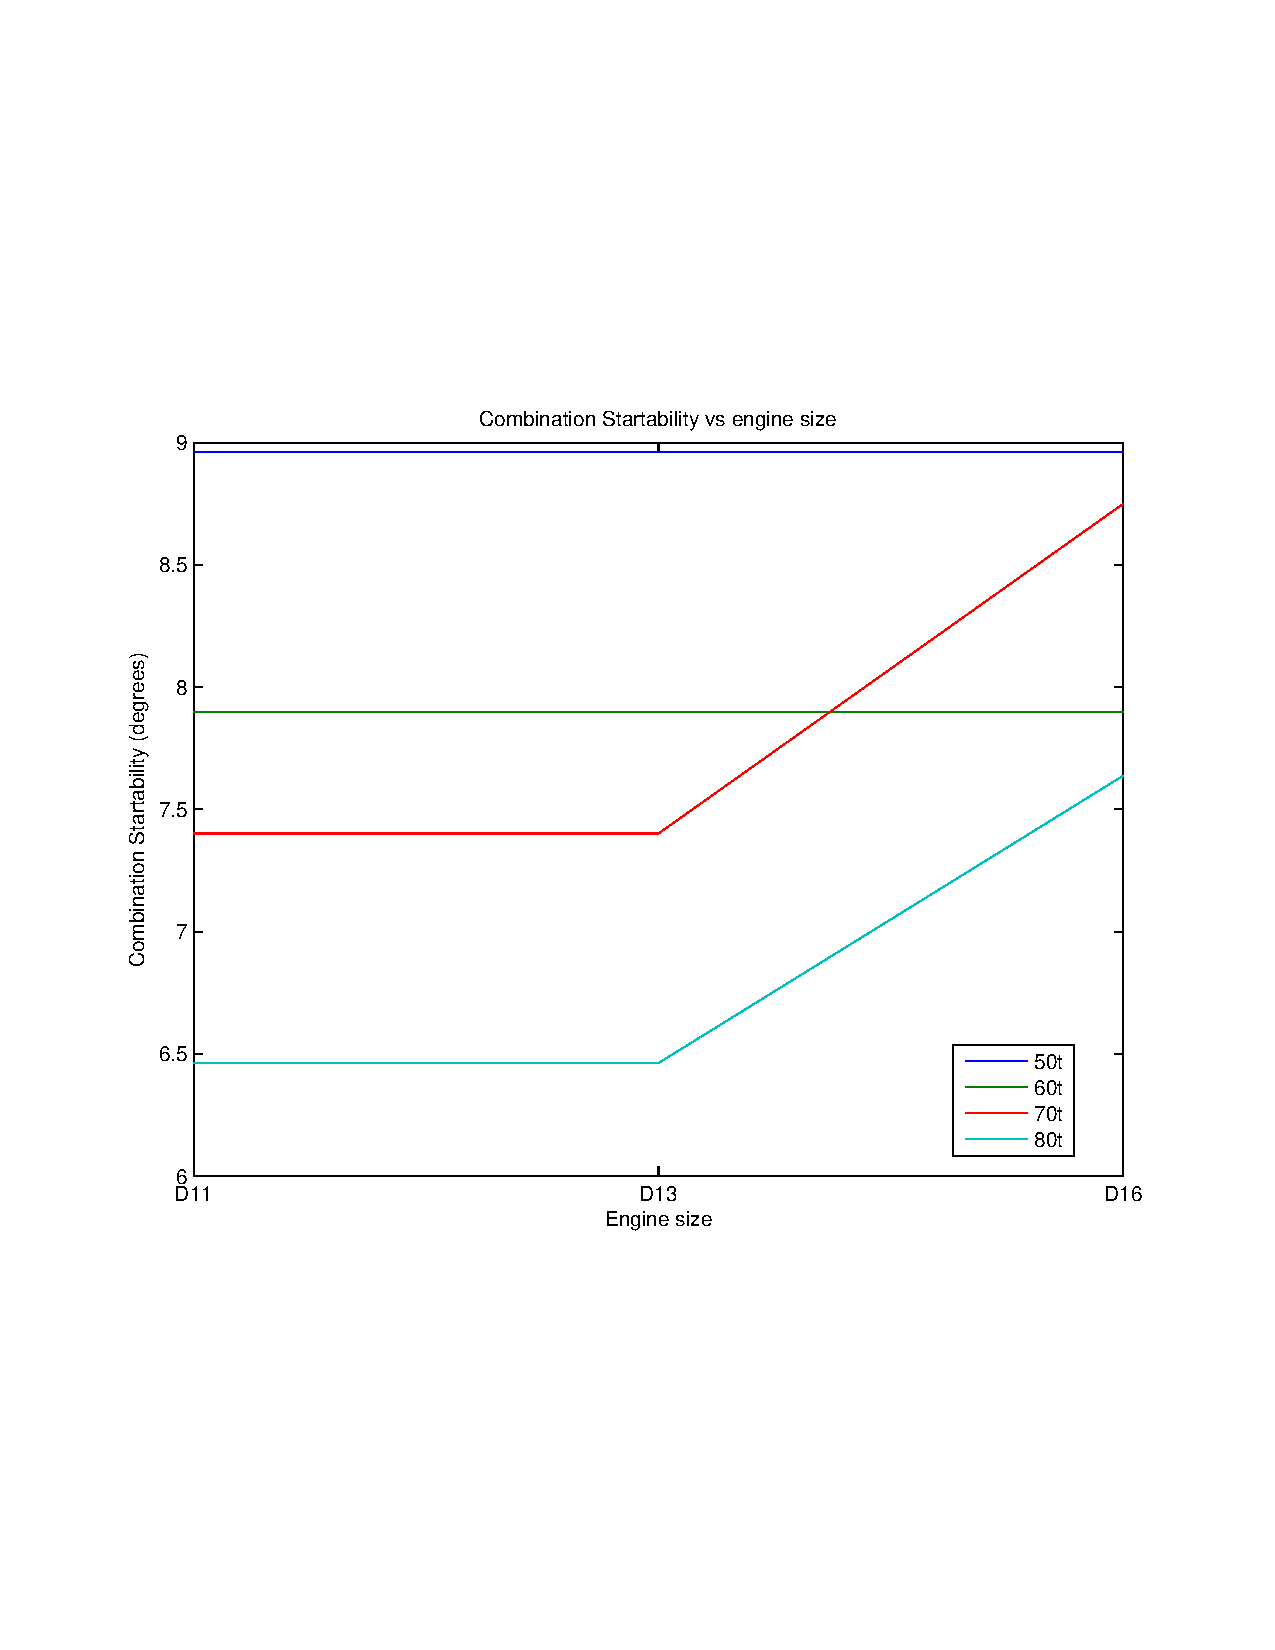
\includegraphics[width=0.5\linewidth, clip=true, trim=45 185 65 208]{figures/ModelValidation/Engine_size_and_GCW/Combination_startability_vs_GCW_and_engine_size.pdf}
\caption{Effect of engine size and GCW on combination startability}
\label{startabilityEngineGCW}
\end{figure}

It should be noted here that the D13 engine shows higher fuel economy than the D11 and D16 engines for the same GCW. The startability of the combinations was also similarly compared as depicted in Figure \ref{startabilityEngineGCW}. Since the combination is traction limited at lower GCWs, the startability is unaffected by engine size for GCWs 50t and 60t. The unchanged startability at higher GCWs between the D11 and D13 combinations can be attributed to the similar starting torques (close to idling engine RPM) of the two engines. It must be noted that this comparison benefits from identical tractor rear axle loads. The influence of axle load on the startability will be examined in a later section.\\

\begin{figure}[h!]
\centering
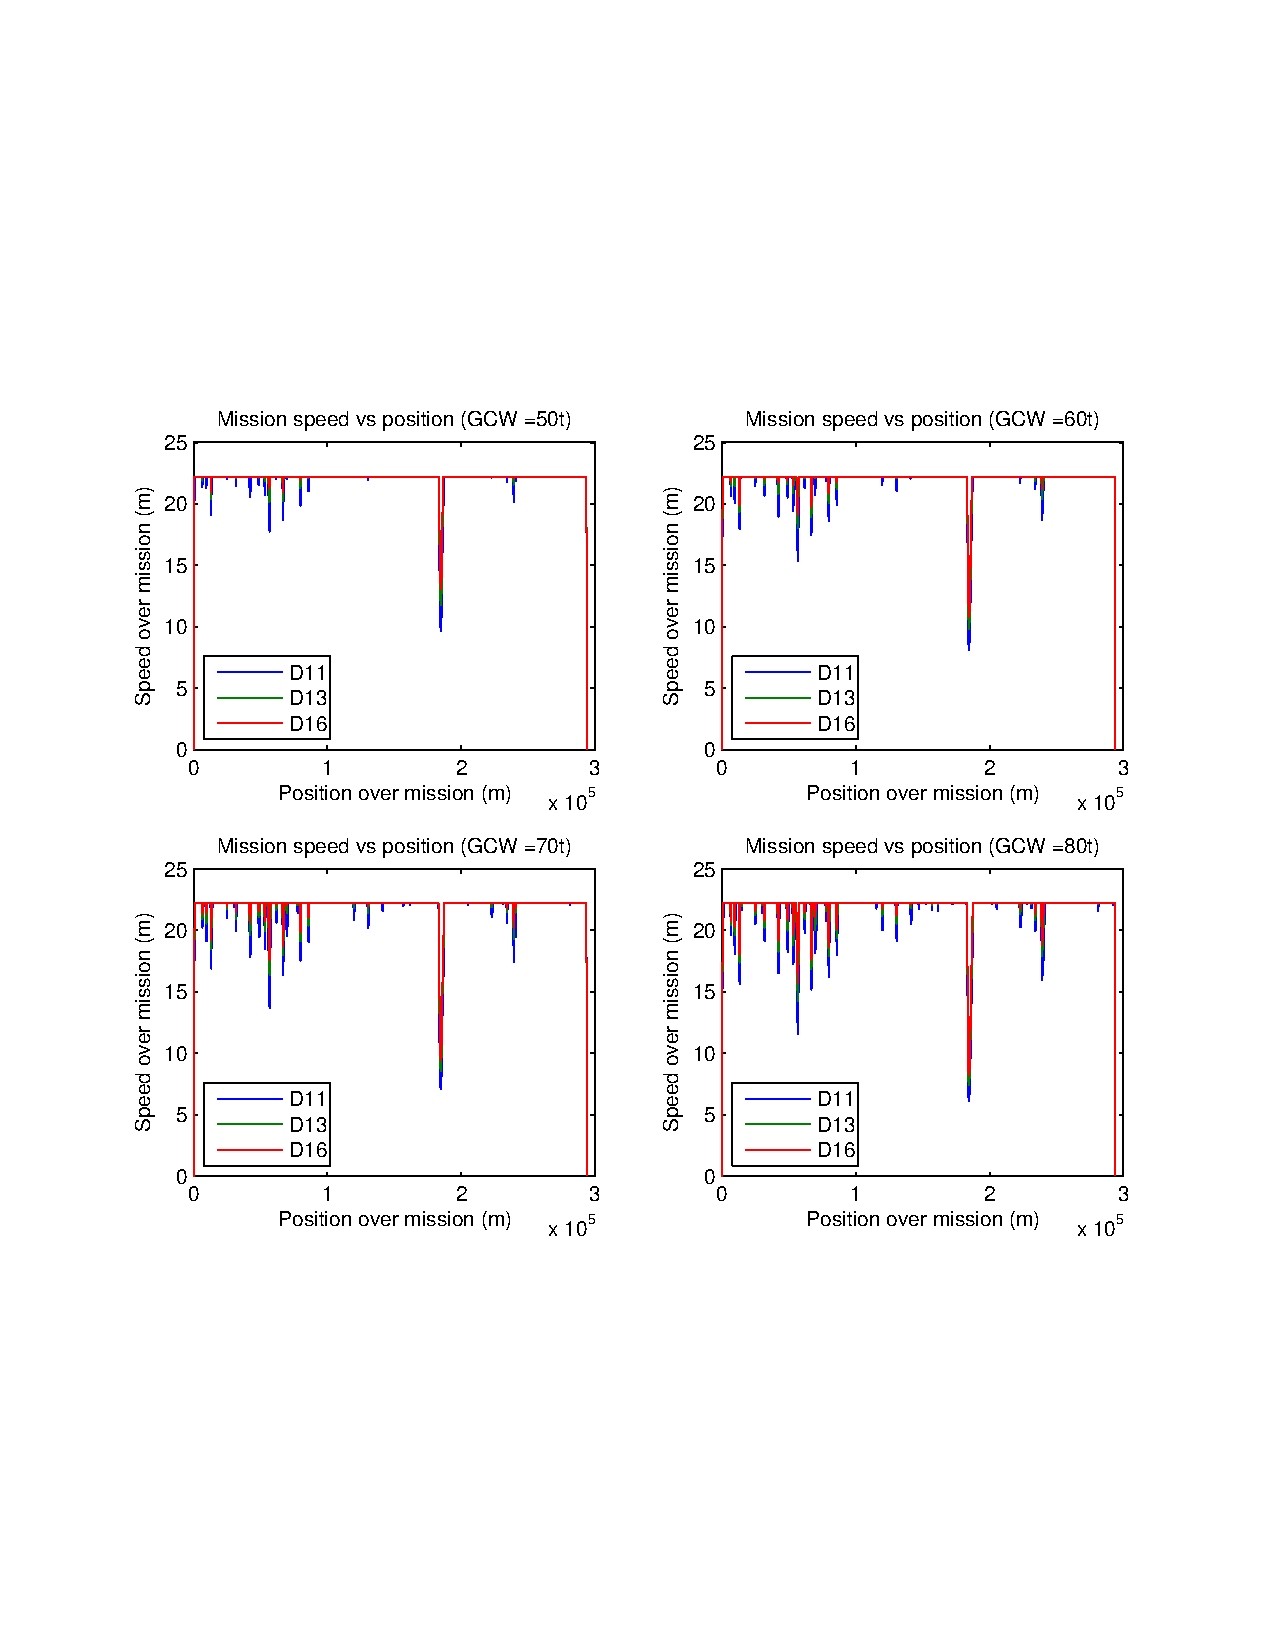
\includegraphics[width=\linewidth, clip=true, trim=45 185 65 208]{figures/ModelValidation/Engine_size_and_GCW/Mission_speed_vs_position.pdf}
\caption{Effect of engine size and GCW on combination speed along the mission}
\label{missionSpeedEngineSizeGCW}
\end{figure}

\begin{figure}[h!]
	\begin{subfigure}{.5\textwidth}
		\centering
		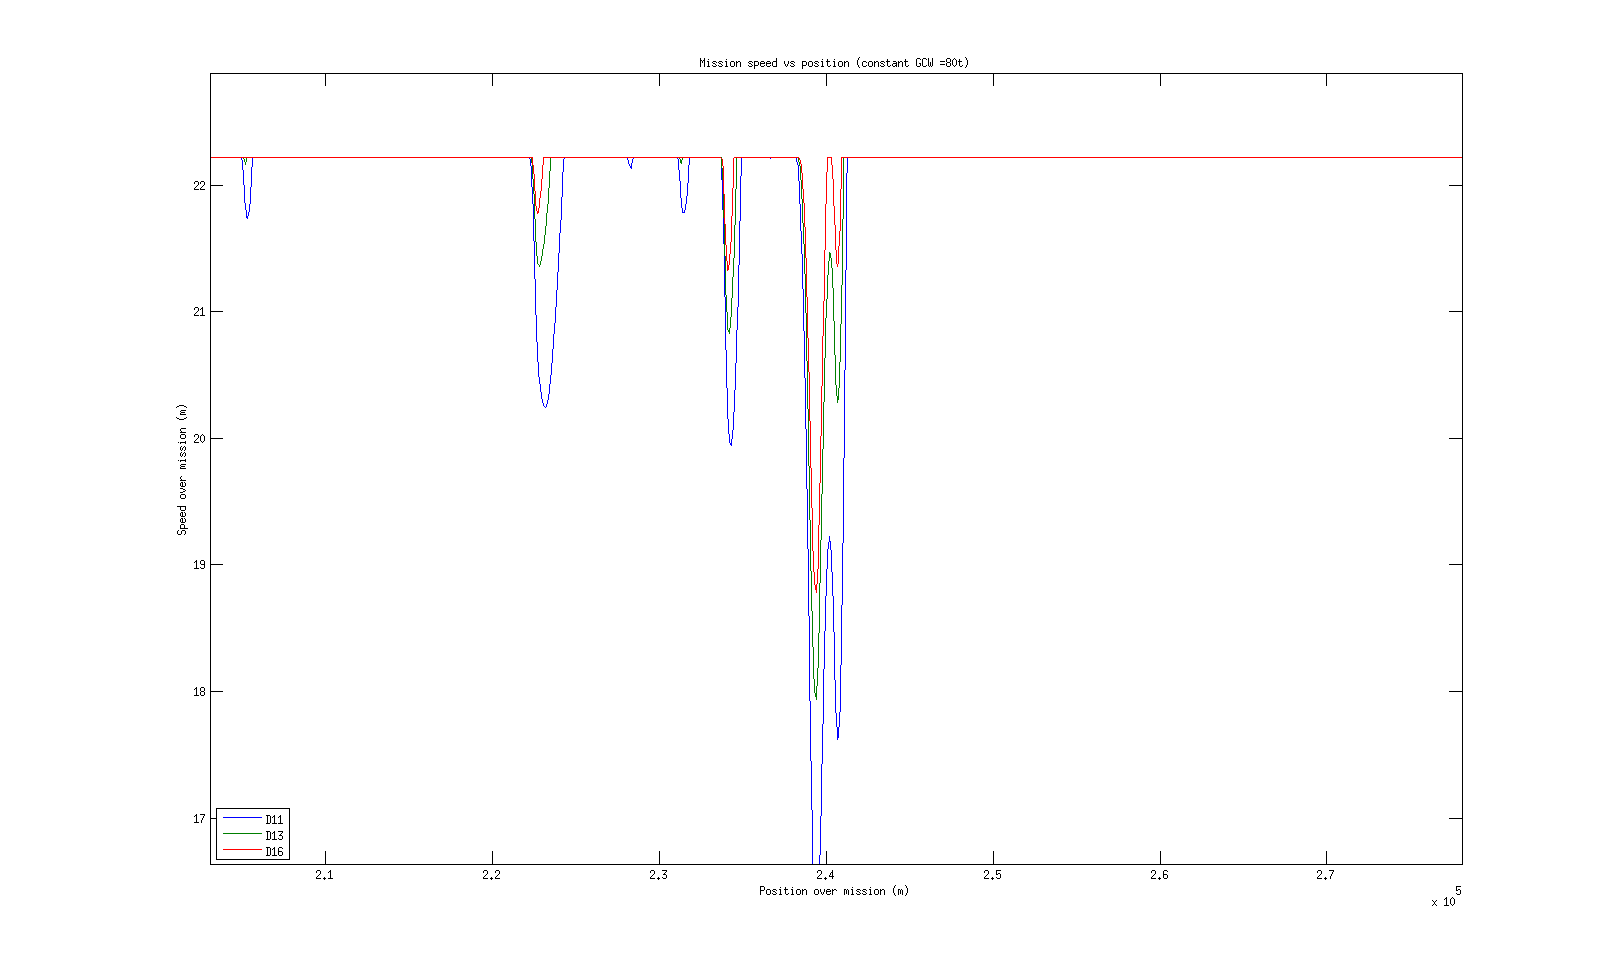
\includegraphics[width=\linewidth]{figures/ModelValidation/Engine_size_and_GCW/MissionSpeed80tZoomed.png}
		\caption{D11 has significantly lower average speeds}
	\end{subfigure}
	\begin{subfigure}{.5\textwidth}
		\centering
		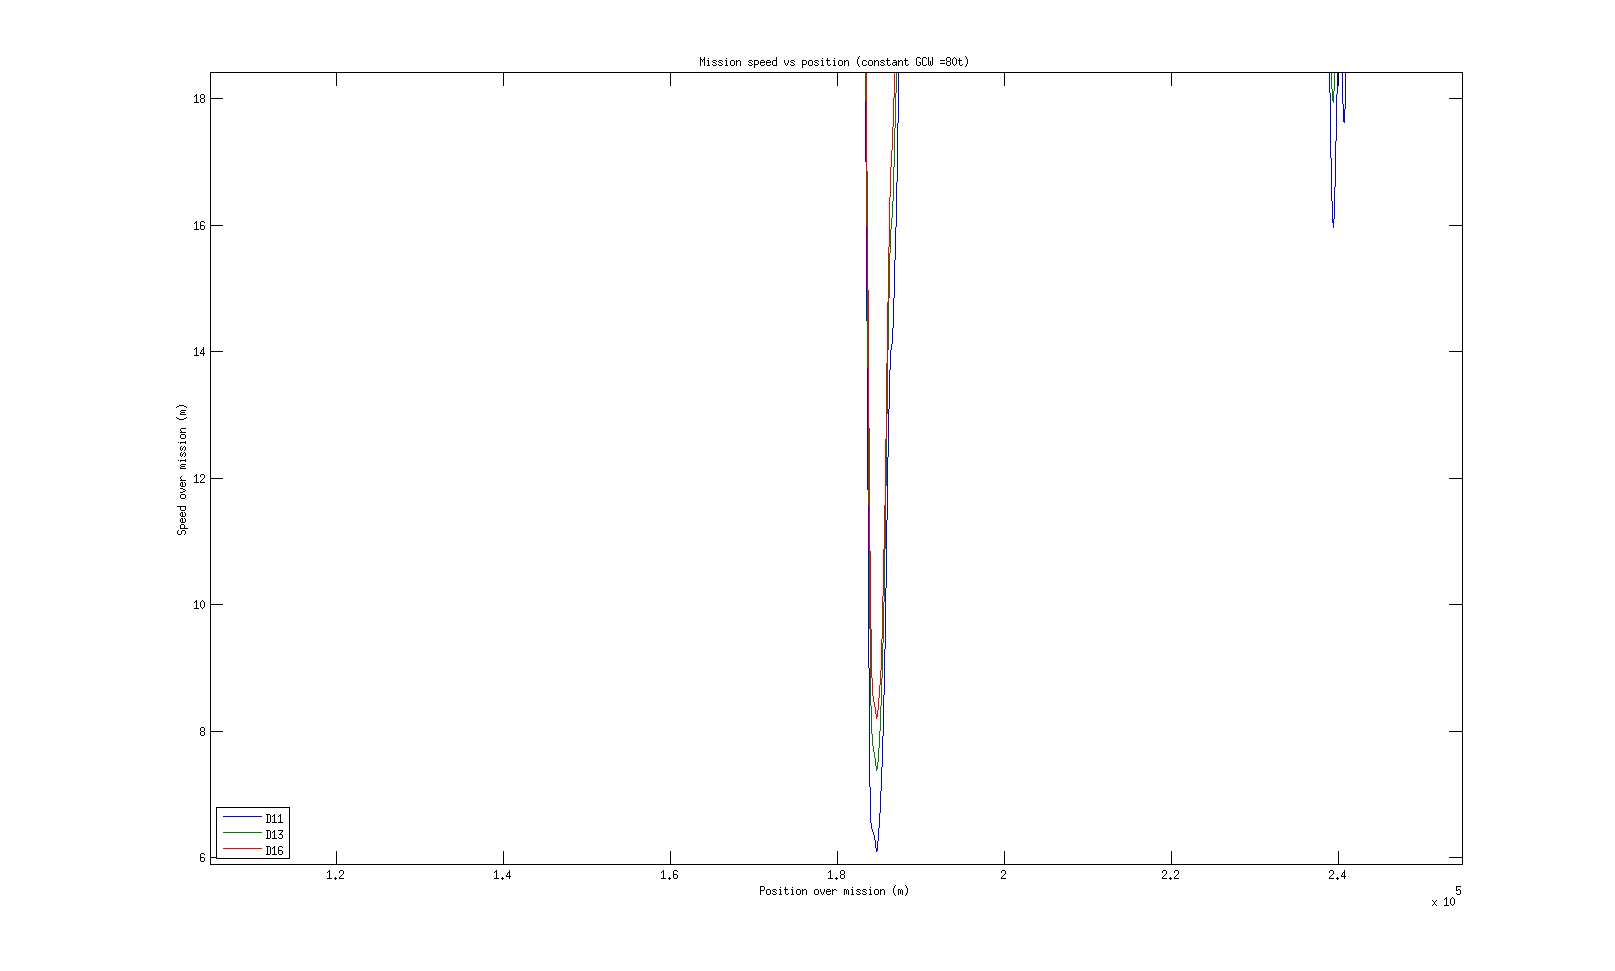
\includegraphics[width=\linewidth]{figures/ModelValidation/Engine_size_and_GCW/MissionSpeed80tZoomedMaxGradient.png}
		\caption{Speed at max altitude (Hallands\aa sen)}
	\end{subfigure}
	\caption{Effect of engine size and GCW on combination speed along the mission}
	\label{zoomedMissionSpeedEngineSizeGCW}
\end{figure}

The speed of the combination along the mission is then recorded and compared among the three engines. This is depicted for all loads in Figure \ref{missionSpeedEngineSizeGCW}. As can be seen, the maximum speed at the top of the highest gradient along the mission reduces with increasing GCW and with engine downsizing. At higher loads, much of the mission along gradients is power limited. The gap in combination performance is hence accentuated at higher loads. A zoomed in view of the combination speed for the combination of GCW 80t is shown in Figure \ref{zoomedMissionSpeedEngineSizeGCW}. The speeds at the crest of the gradient are 7.11ms\textsuperscript{-1}, 8.59ms\textsuperscript{-1} and 9.59ms\textsuperscript{-1} for the combinations powered by the D11, D13 and D16 engines respectively.\\

The combination with the D11 engine thus decelerates the most, up the gradient at Hallands\aa sen. It can also be seen from the plots that the combination with D16 engine begins deceleration the latest and quickly recovers the target speed thus maintaining a sizeably higher average speed over the D11 and D13 combinations.

\subsection{Number of axles propelled}

The conundrum of increasing the number of propelled axles correlates directly with the axle load distribution and road surface. Hence, increasing propulsive power improves mission startability and average speed only upto a point beyond which the traction limits of the road make the excess power unusable. This progressive improvement and the performance cusp is investigated here. The common GCW considered is 68t.\\

\begin{figure}[h!]
\begin{subfigure}{.5\textwidth}
	\centering
	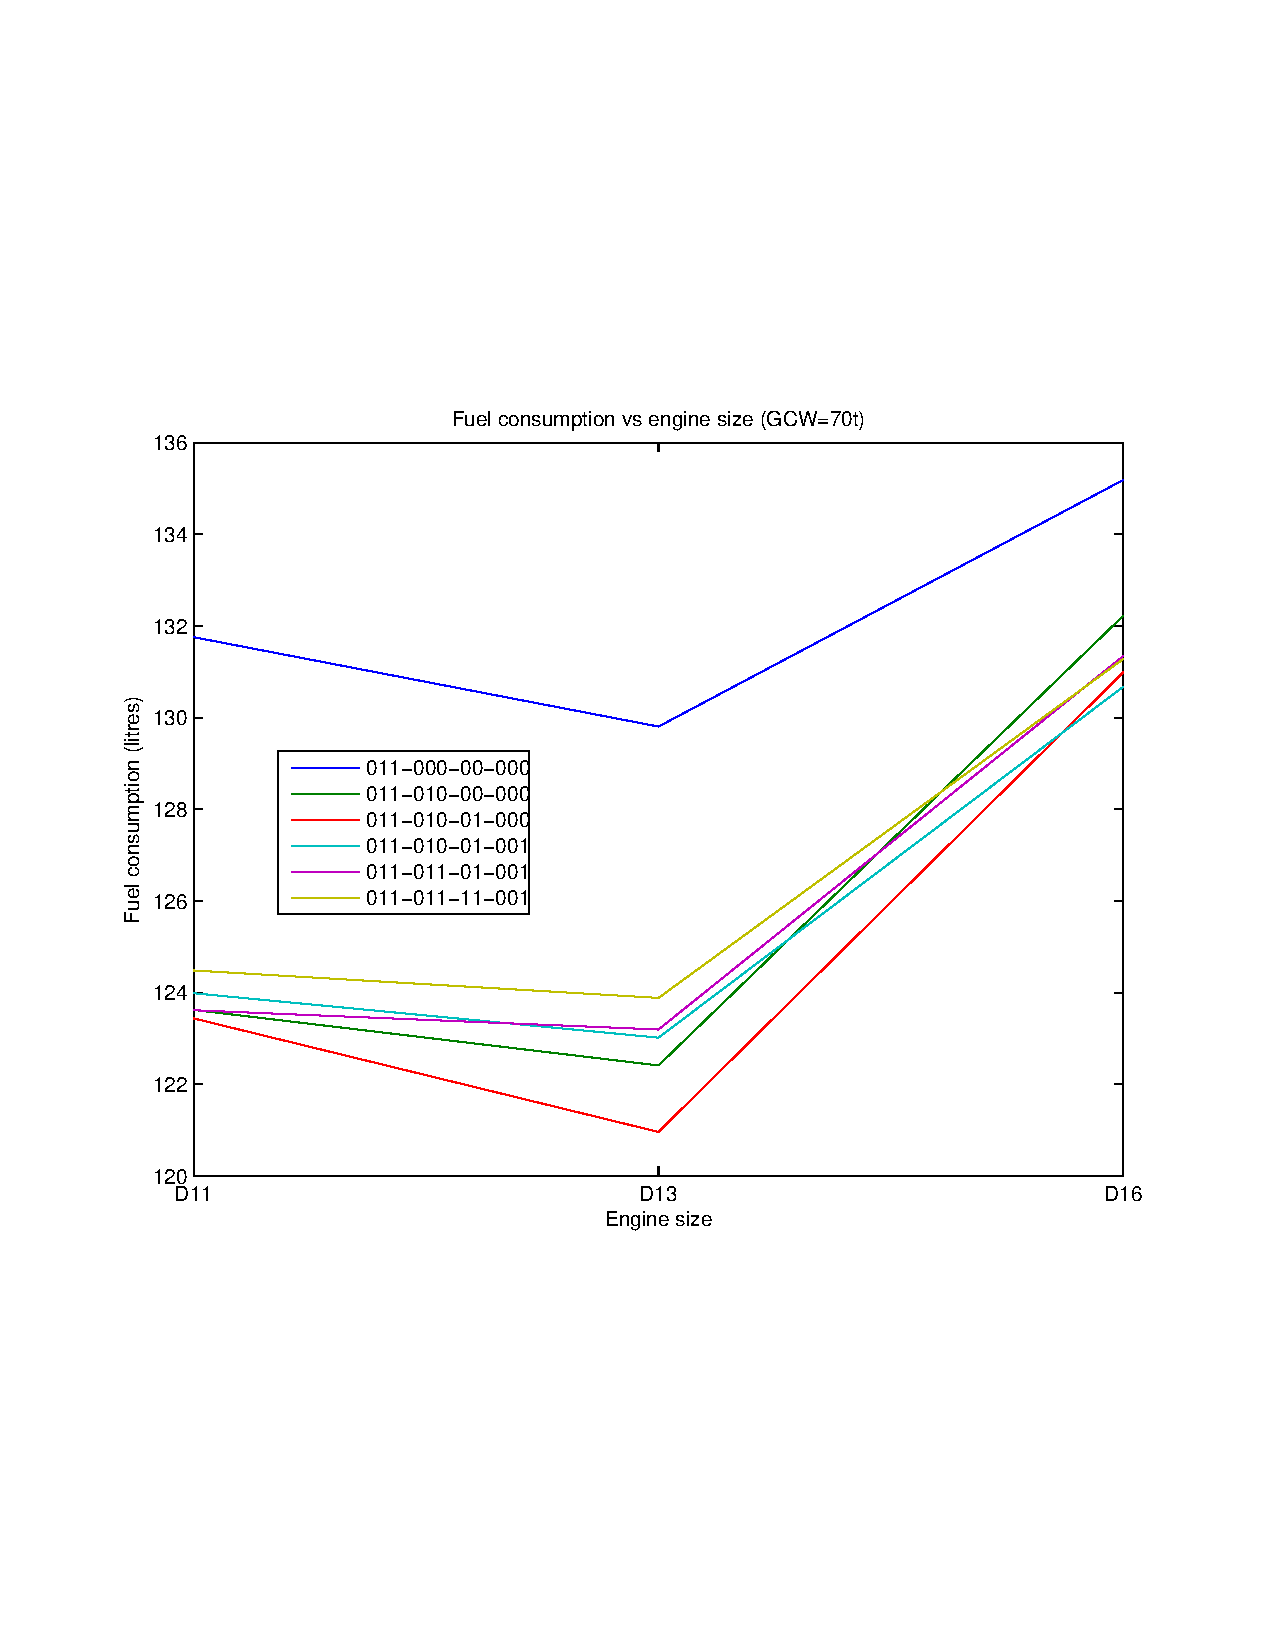
\includegraphics[width=\linewidth, clip=true, trim=45 185 65 208]{figures/ModelValidation/Increasing_number_of_axles/Fuel_consumption_vs_axle_number_and_engine_size.pdf}
	\caption{Fuel consumption over mission}
\end{subfigure}
\begin{subfigure}{.5\textwidth}
	\centering
	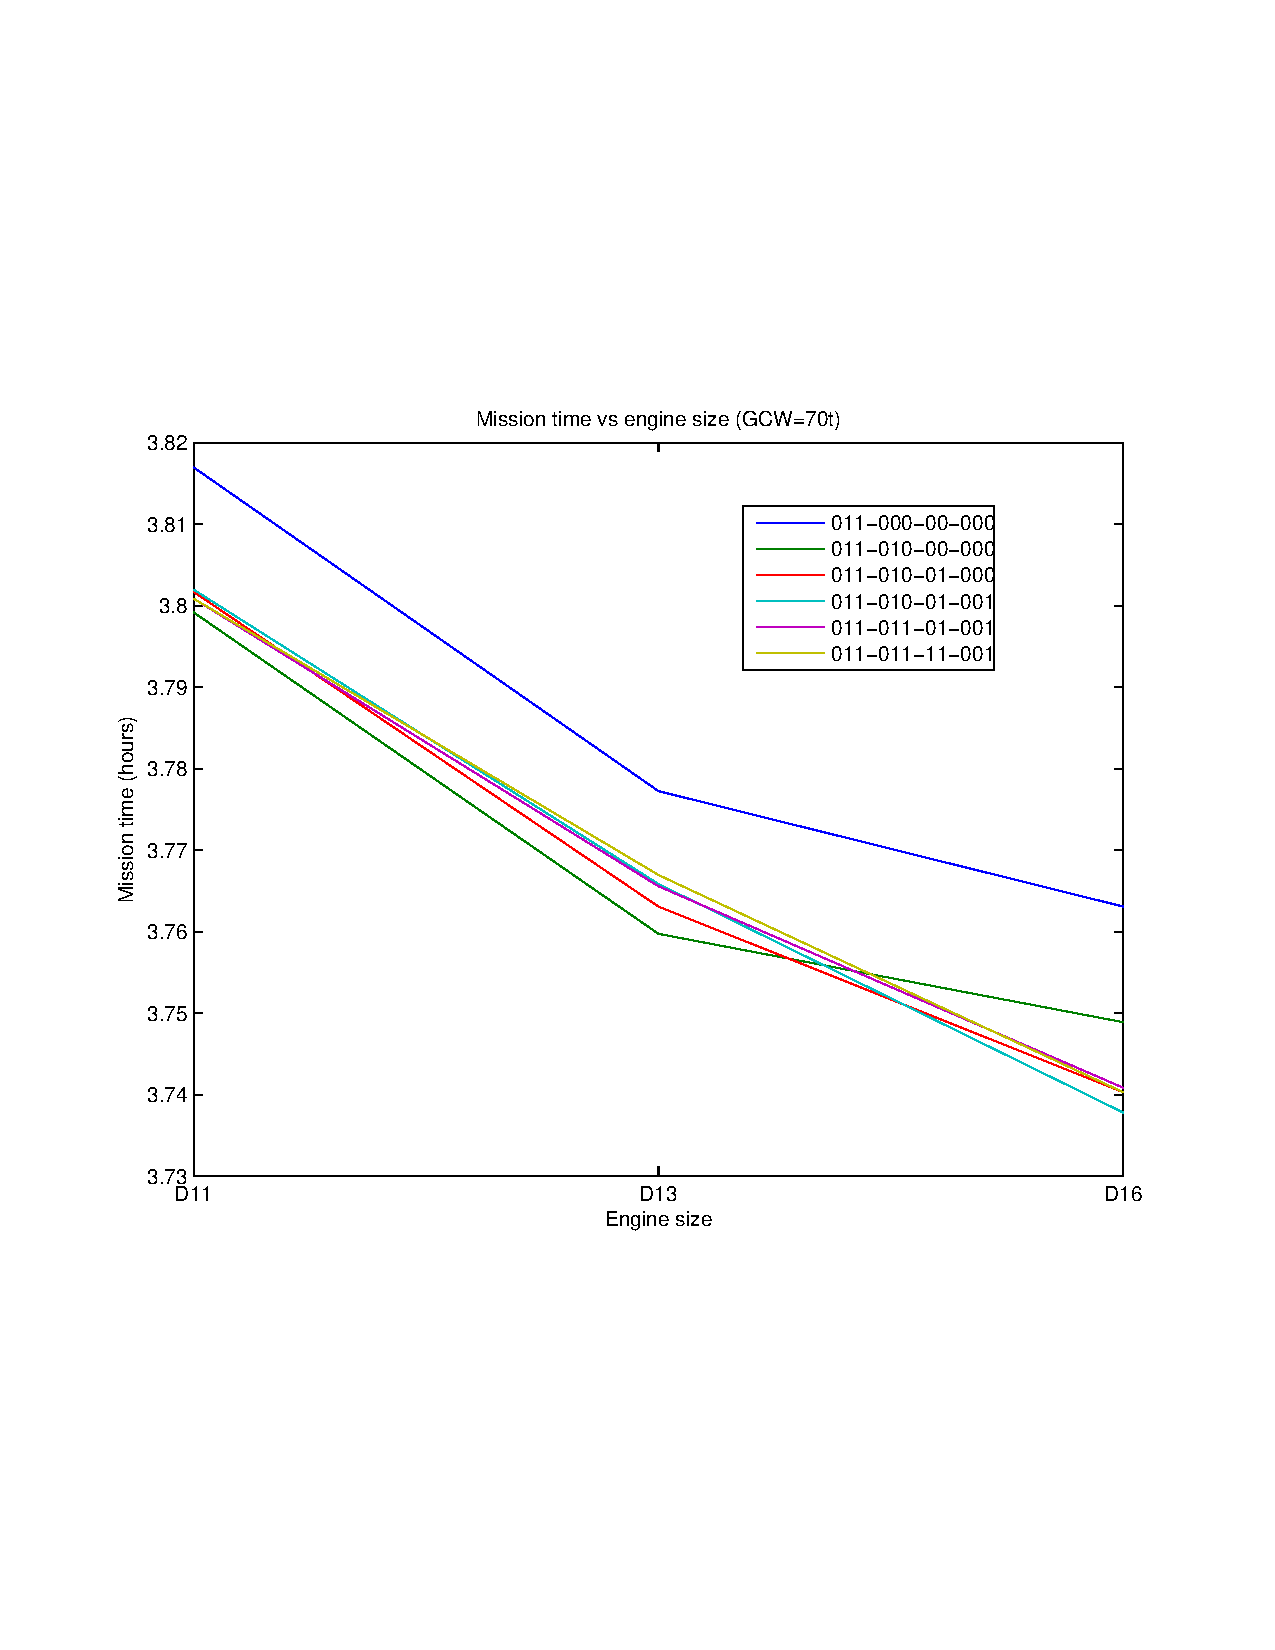
\includegraphics[width=\linewidth, clip=true, trim=45 185 65 210]{figures/ModelValidation/Increasing_number_of_axles/Mission_time_vs_axle_number_and_engine_size.pdf}
	\caption{Mission time}
\end{subfigure}
\caption{Effect of number of propelled axles \& engine size on fuel consumption and mission time}
\label{timeFuelNumberOfAxlesEngine}
\end{figure}

It can be noticed here, as depicted in Figure \ref{timeFuelNumberOfAxlesEngine}, taking the D13 combination in specific, that the fuel consumption reduces while increasing the number of propelled axles to 1 and 2 consecutively. Thereafter, additional propulsion adversely affects fuel consumption, though, of course, staying significantly below the pure combustion combination. This can be attributed to the energy management strategy employed in the vehicle model. When fewer axles are propelled, the demanded power frequently exceeds the maximum tractive power that the combination provides allowing the motors to operate at their maximum tractive potential. When the number of propelled axles is increased, the algorithm seeks to run the engine at its optimum operating point more often while only distributing the remaining power demand to the motors. This explains the increase in engine usage and the consecutive increase in fuel consumption and mission time when the number of propelled axles is increased beyond 2. The percentage reductions in fuel consumption are tabulated in Table \ref{table:fuelConsumptionReductionAxles}.\\

The mere addition of a single electrically propelled axle (173kW \& 411Nm electric motor for each propelled axle and 5.98MC buffer for each respective unit) on the D11 engine-only combination yields a 6.2\% reduction in fuel consumption while the potential savings are significantly improved in the case of the D13 combinations. Savings of upto 9.9\% compared to the engine-only combinations are seen with the addition of one propelled axle each on every trailing unit. Observing the trends in the D16 combinations clearly show successive increases in fuel consumption upto a point where the engine optimum operation trend mitigates the savings to around 3\%. This substantiates the motivation rendered earlier.\\

\begin{table}[h!]
\centering
\begin{tabular}{|c|c|c|c|c|c|c|}
\hline
& 011-010-00-000 & 011-010-01-000 & 011-010-01-010 & 011-011-01-010 & 011-011-11-010 \\
\hline
D11 & 6.17 & 6.31 & 5.89 & 6.17 & 5.52 \\
\hline
D13 & 5.69 & 6.81 & 9.9 & 5.09 & 4.56 \\
\hline
D16 & 2.19 & 3.1 & 3.34 & 2.84 & 2.89 \\
\hline
\end{tabular}
\caption{Percentage reduction in fuel consumption compared to standard A-Double}
\label{table:fuelConsumptionReductionAxles}
\end{table}

\begin{figure}[h!]
\centering
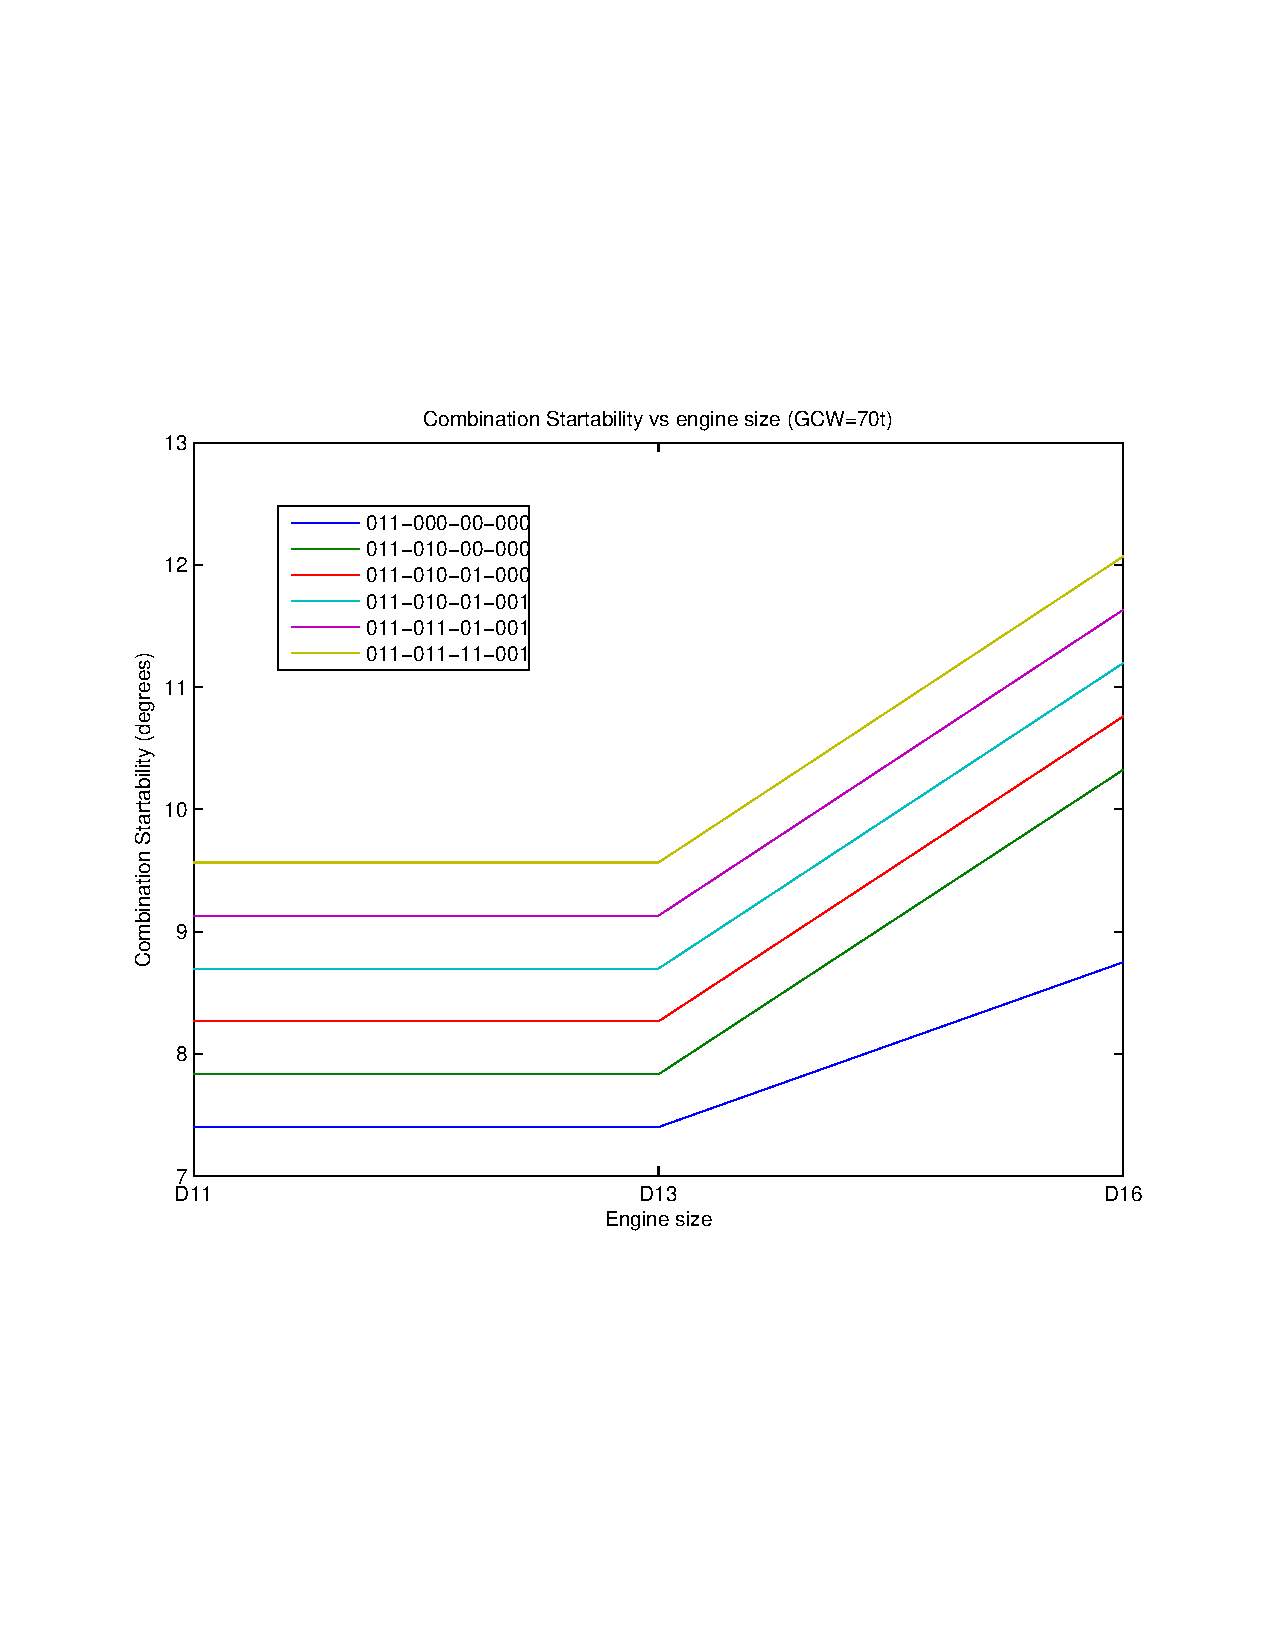
\includegraphics[width=0.5\linewidth, clip=true, trim=45 185 65 208]{figures/ModelValidation/Increasing_number_of_axles/Combination_startability_vs_axle_number_and_engine_size.pdf}
\caption{Effect of engine size and number of propelled axles on combination startability}
\label{startabilityEngineNumberOfAxles}
\end{figure}

The startability of the combination is analysed in a manner similar to before to establish the effect of increased tractive power and is as shown in Figure \ref{startabilityEngineNumberOfAxles}. It must be noted that the rating of the electric motors was maintained constant while simulation combinations with increased number of propelled axles. Hence, the addition of electric machines to the combination results in equally spaced steps on increased startability. Also, as stated before, the identical starting torques of the D11 and D13 engines coupled with the use of similar motors results in the startability of the two combinations remaining similar in each propelled axle configuration case.\\

With a constant GCW of 70t, the effect of increasing electric propulsion on the mission speed is shown in Figure \ref{globalMissionSpeedIncreasedPropulsion}. The delay in the beginning of combination deceleration with increased propulsion and the increased minimum speed at the peak of Hallands\aa sen is clearly seen in Figure \ref{missionSpeedIncreasedPropulsion}. While the pure combustion combination achieves a speed of 9.45ms\textsuperscript{-1}, the addition of one electrically propelled axle increases this speed to 10.42ms\textsuperscript{-1} which is further improved to 11.22ms\textsuperscript{-1} with the addition of another electrically propelled axle. It must be noted that this increase in minimum speed alone cannot be directly attributed to the addition of propulsion since the traction available uphill also depends on the buffer states and efficiencies. Nevertheless, while the buffers are 'available' in this segment, the effect of addition of propulsion is patently evident. The charge consumption in each of the cases is shown in Figure \ref{chargeEngineSizeNumberOfAxles}.\\

\begin{figure}[h!]
\centering
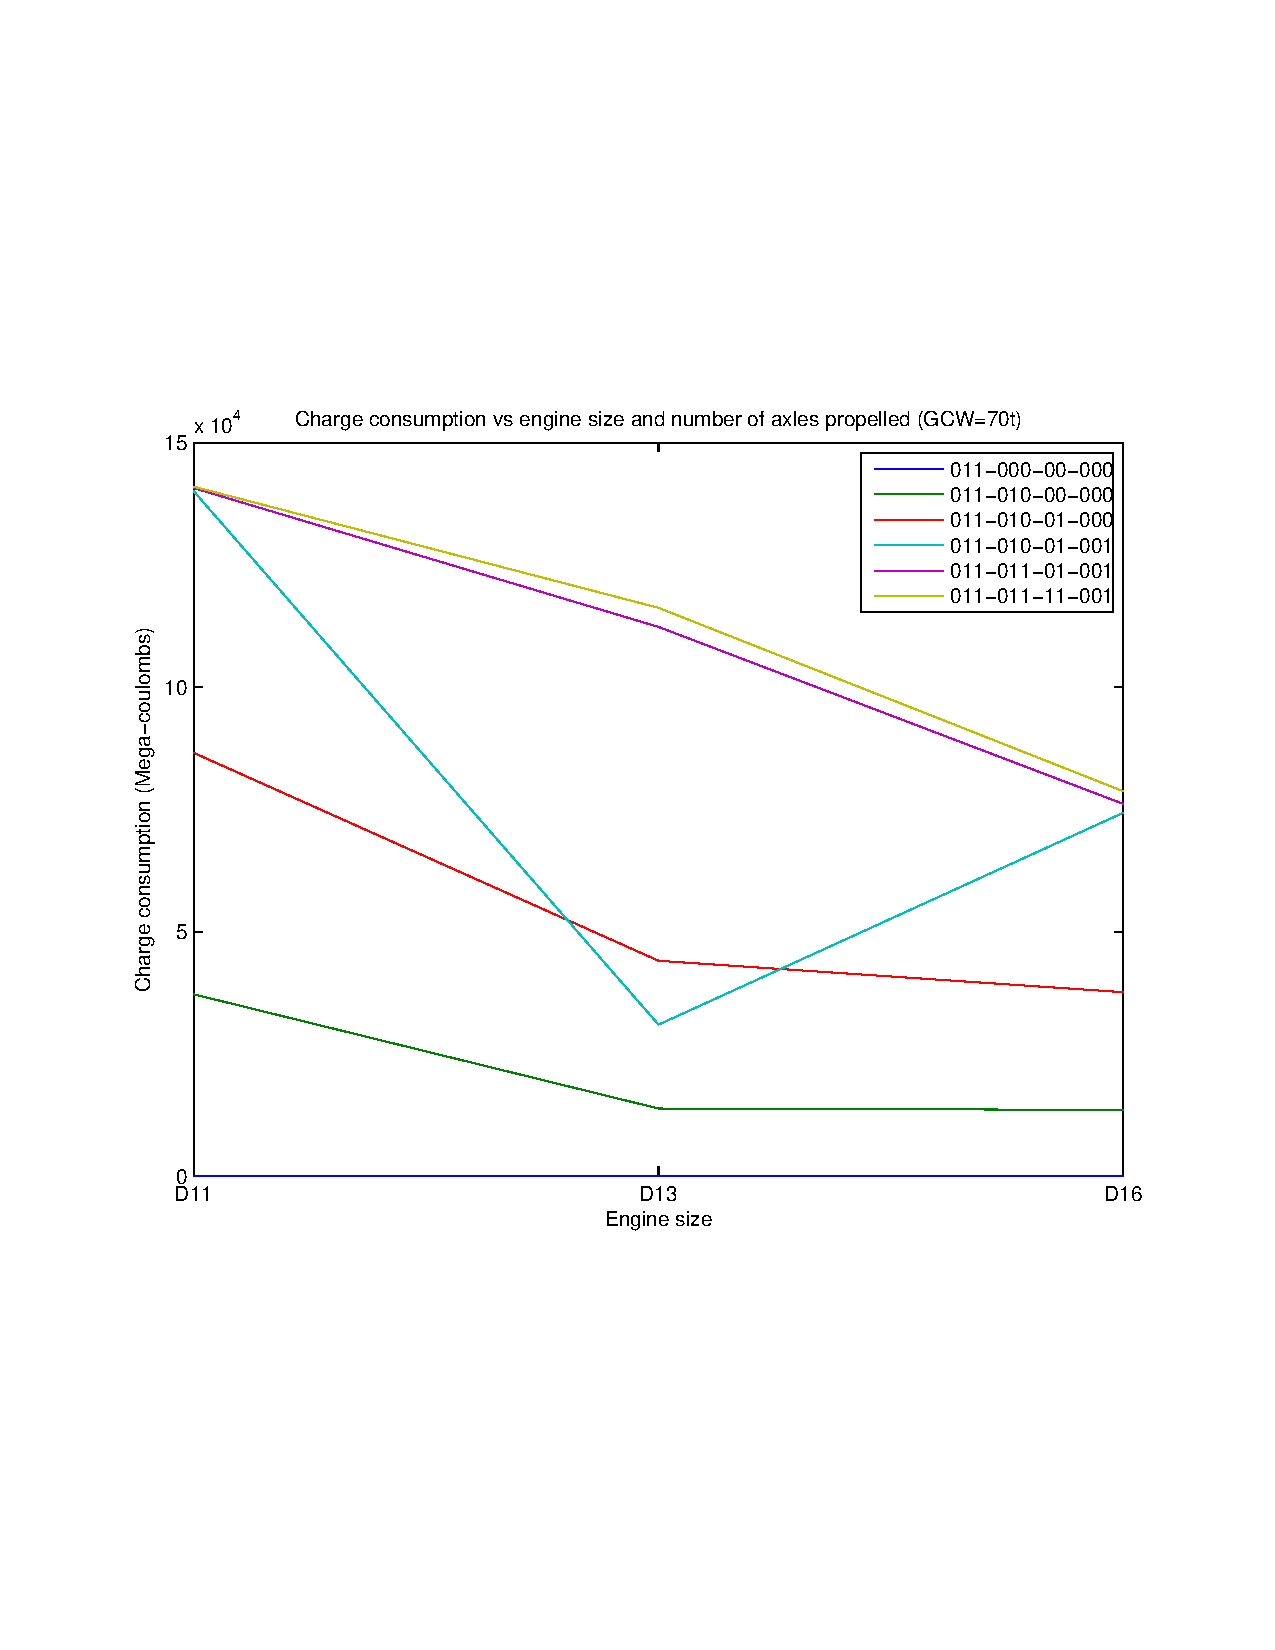
\includegraphics[width=0.5\linewidth, clip=true, trim=45 185 65 208]{figures/ModelValidation/Increasing_number_of_axles/Charge_consumption_vs_axle_number_and_engine_size.pdf}
\caption{Effect of engine size and number of propelled axles on charge consumption}
\label{chargeEngineSizeNumberOfAxles}
\end{figure}

\begin{figure}[h!]
\centering
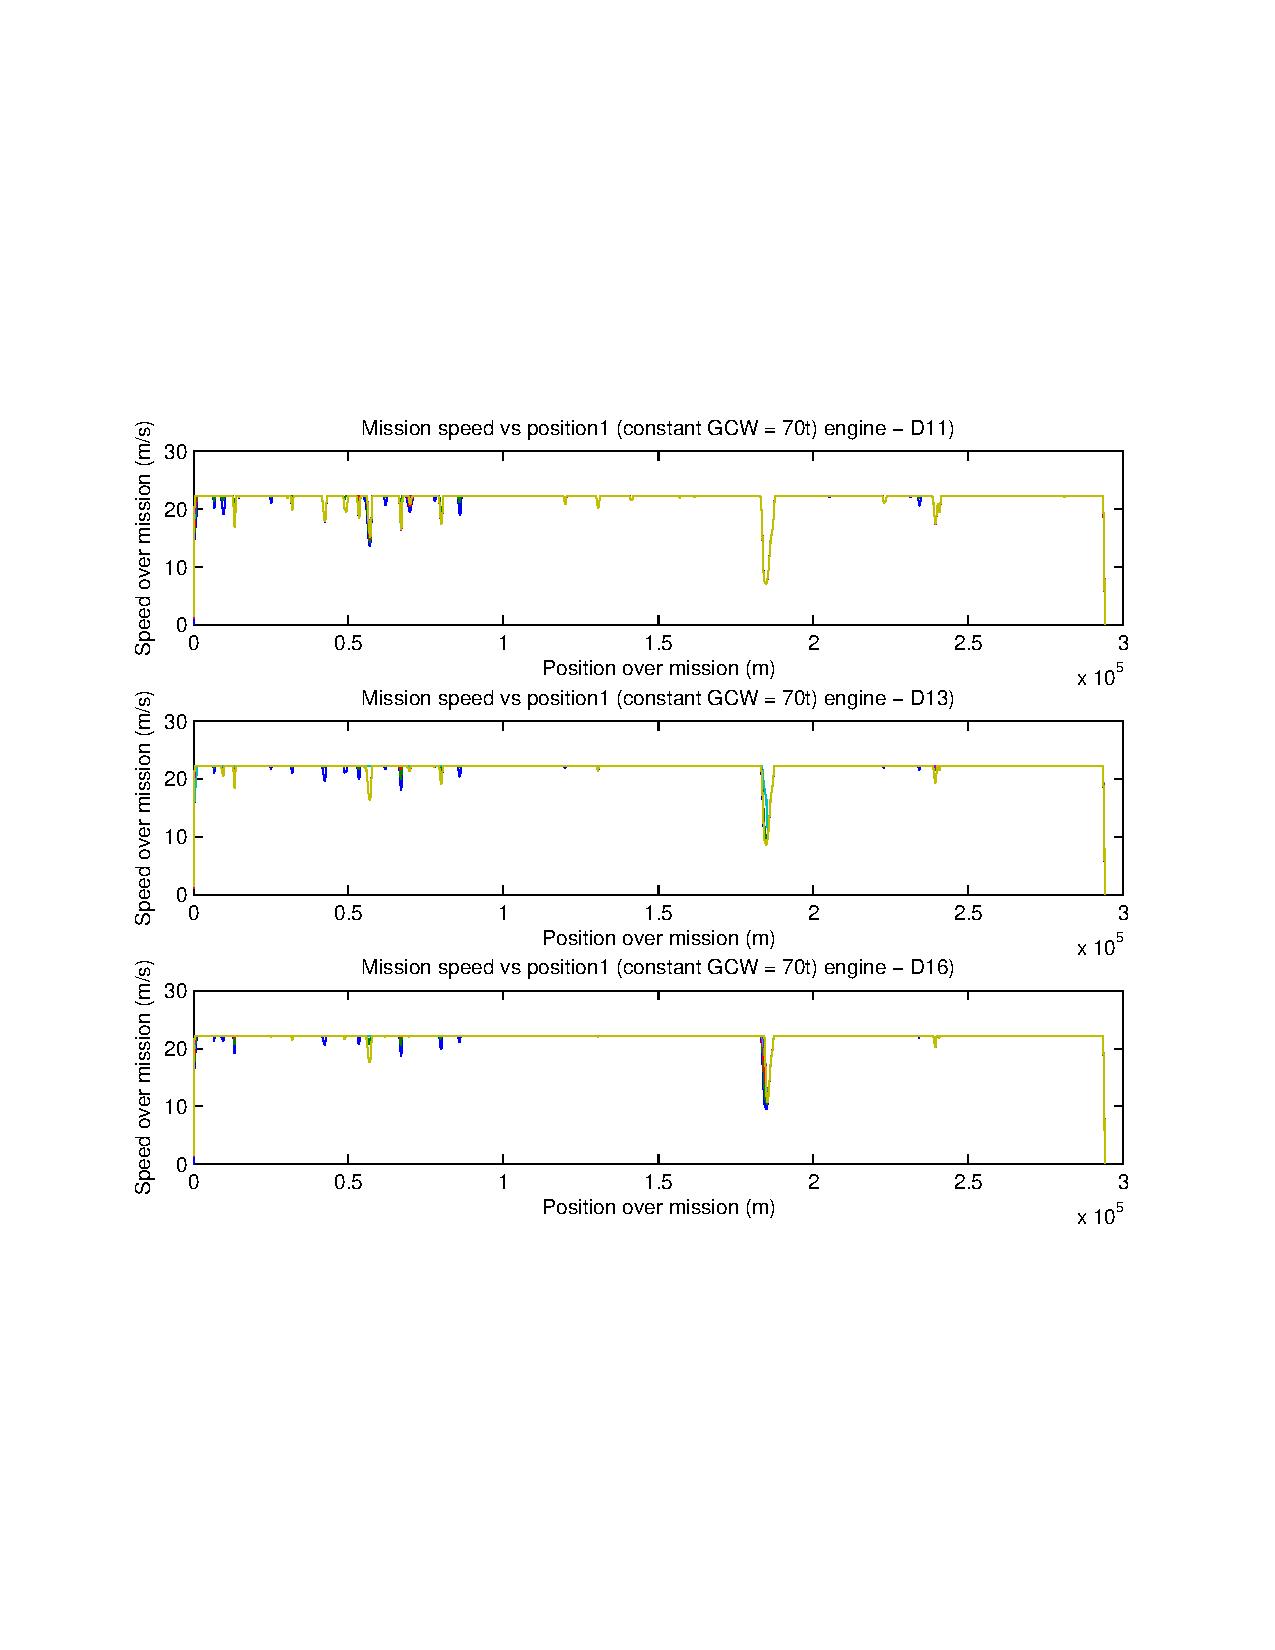
\includegraphics[width=\linewidth, clip=true, trim=45 185 65 200]{figures/ModelValidation/Increasing_number_of_axles/Mission_speed_vs_position_(constant_GCW=70t).pdf}
\caption{Increased propulsion and its influence on mission speed}
\label{globalMissionSpeedIncreasedPropulsion}
\end{figure}

\begin{figure}[h!]
\begin{subfigure}{.5\textwidth}
	\centering
	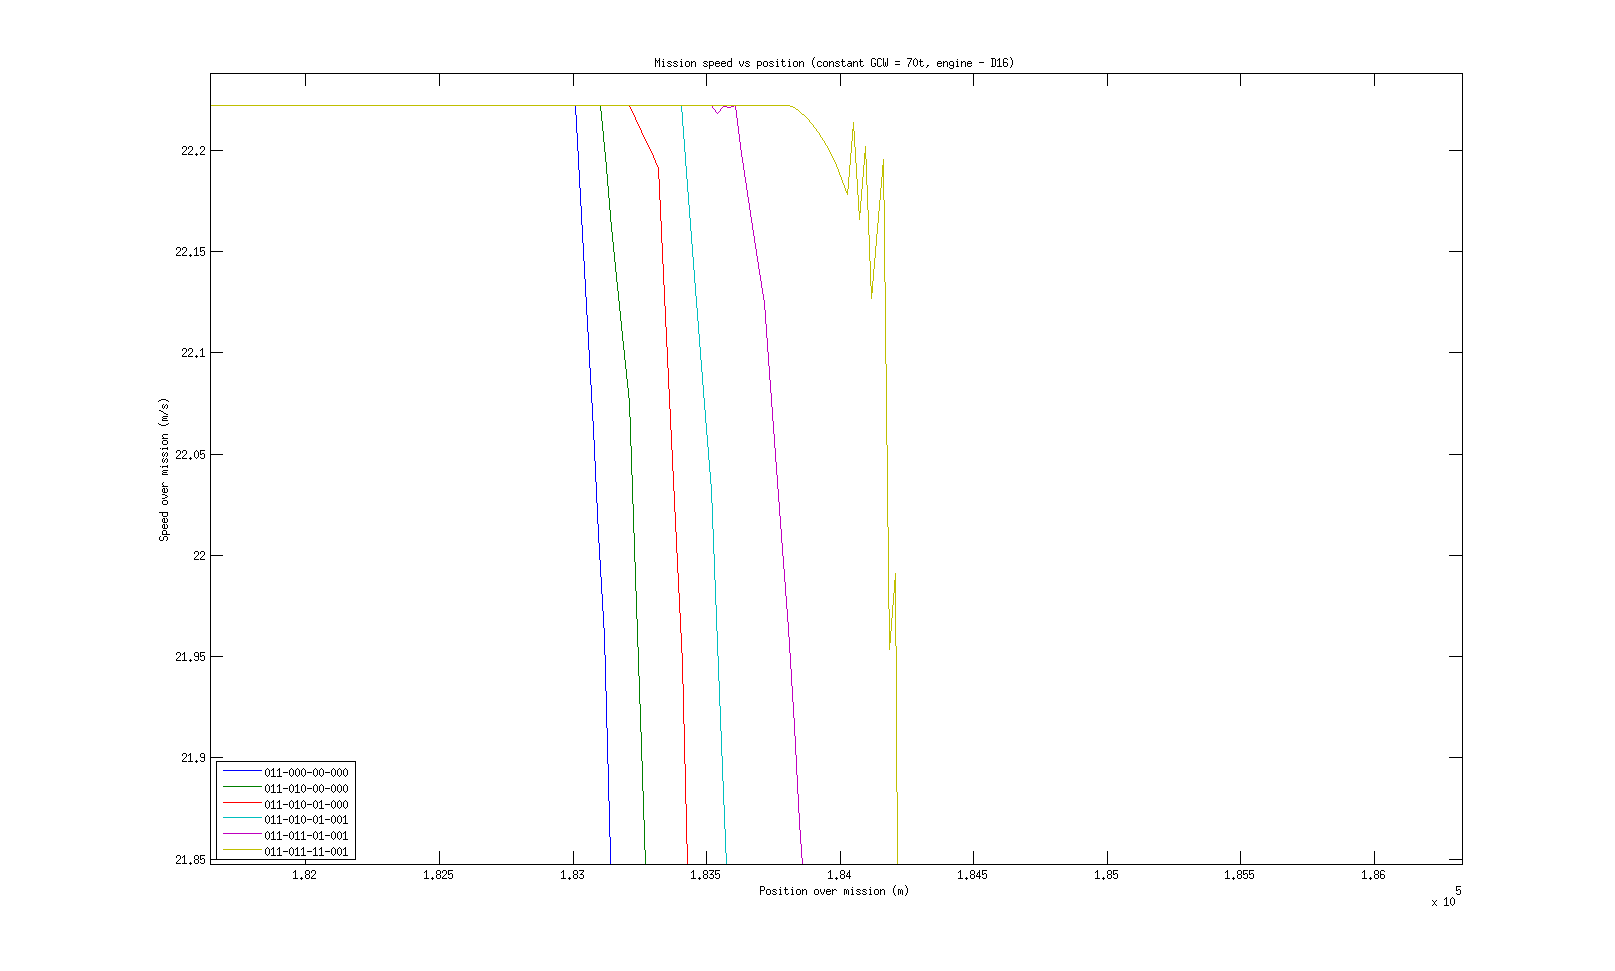
\includegraphics[width=\linewidth]{figures/ModelValidation/Increasing_number_of_axles/Speed_vs_position_zoomed_no_of_axles_begin_dec.png}
	\caption{Vehicle speed at the beginning of Hallands\aa sen}
\end{subfigure}
\begin{subfigure}{.5\textwidth}
	\centering
	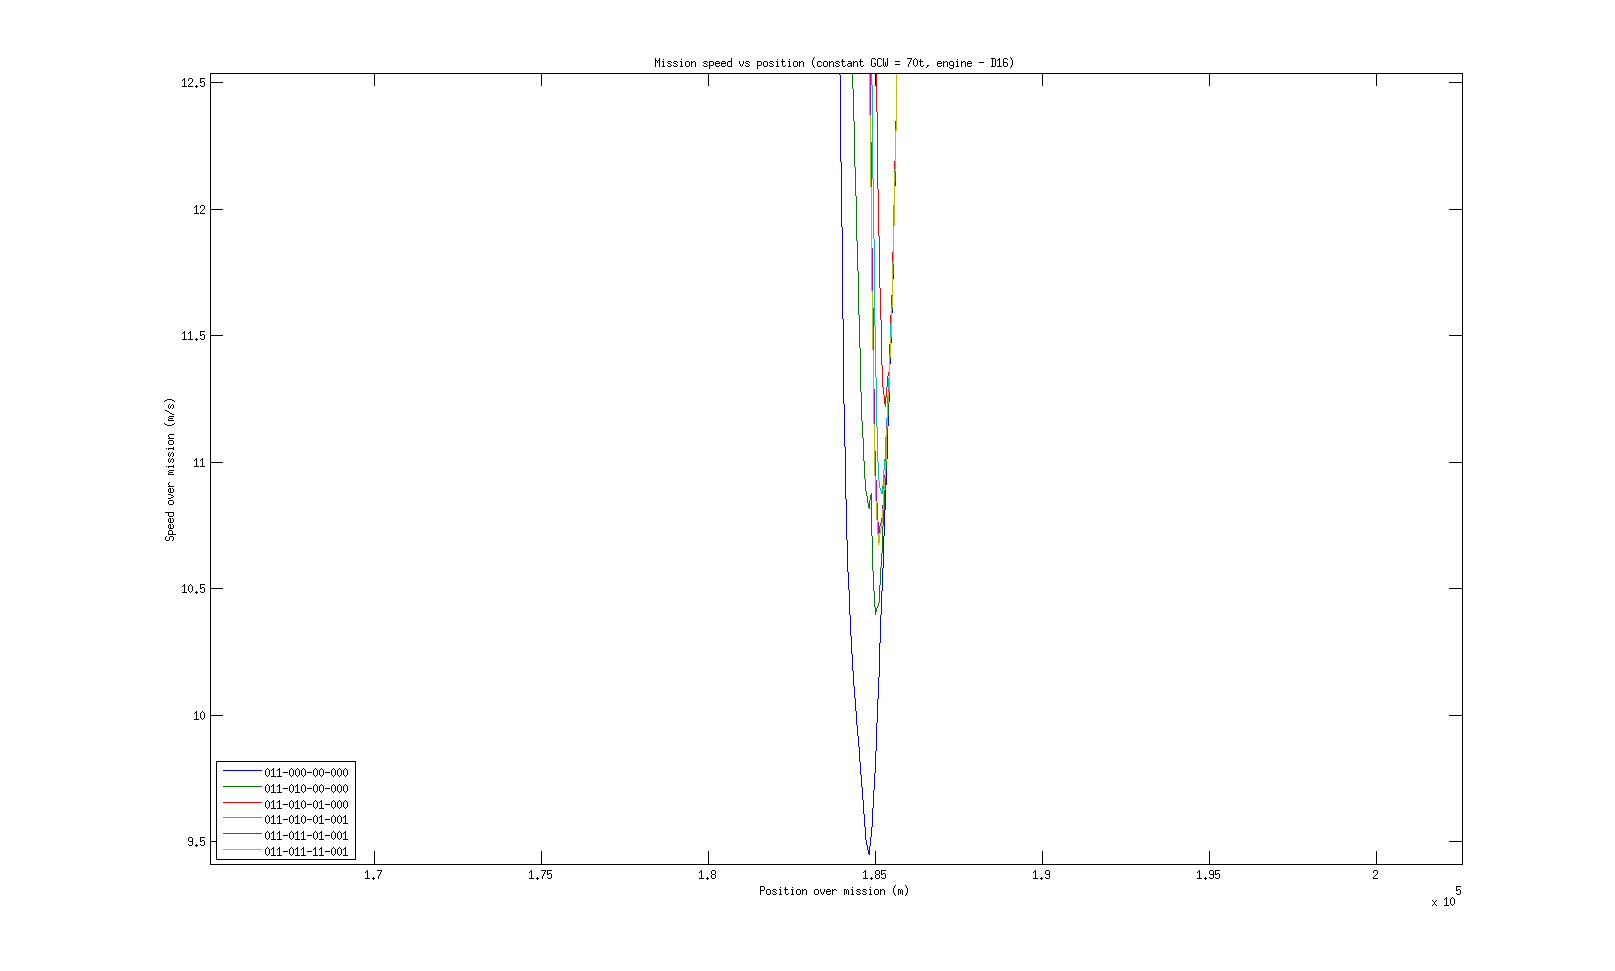
\includegraphics[width=\linewidth]{figures/ModelValidation/Increasing_number_of_axles/Speed_vs_position_zoomed_no_of_axles_peak.png}
	\caption{Speed at the peak of Hallands\aa sen}
\end{subfigure}
\caption{Effect of number of propelled axles on mission speed}
\label{missionSpeedIncreasedPropulsion}
\end{figure}

\subsection{Axle load}

The axle load of propelled axles determines the useability of the traction that the motor provides. When presented with the problem of choosing a specific number or combination of axles to be propelled given a specified number of electric machines, the choice of axles must be preferential with higher axle loads. This is inspected by assigning an electric machine alternatively to three different axles with varying axle loads and observing the mission performance. Each axle on the first semitrailer, dolly and the second semitrailer in the A-Double combination carry 7.3t, 5.25t and 4.49t respectively. Hence, in each of the simulations performed, a single axle on one of the three trailing units is chosen to be propelled. A constant GCW of 70t is assigned.\\

The fuel consumption and mission time in each of the cases is depicted in Figure \ref{fuelTimeEngineAxleLoad}. 

\begin{figure}[h!]
\begin{subfigure}{.5\textwidth}
	\centering
	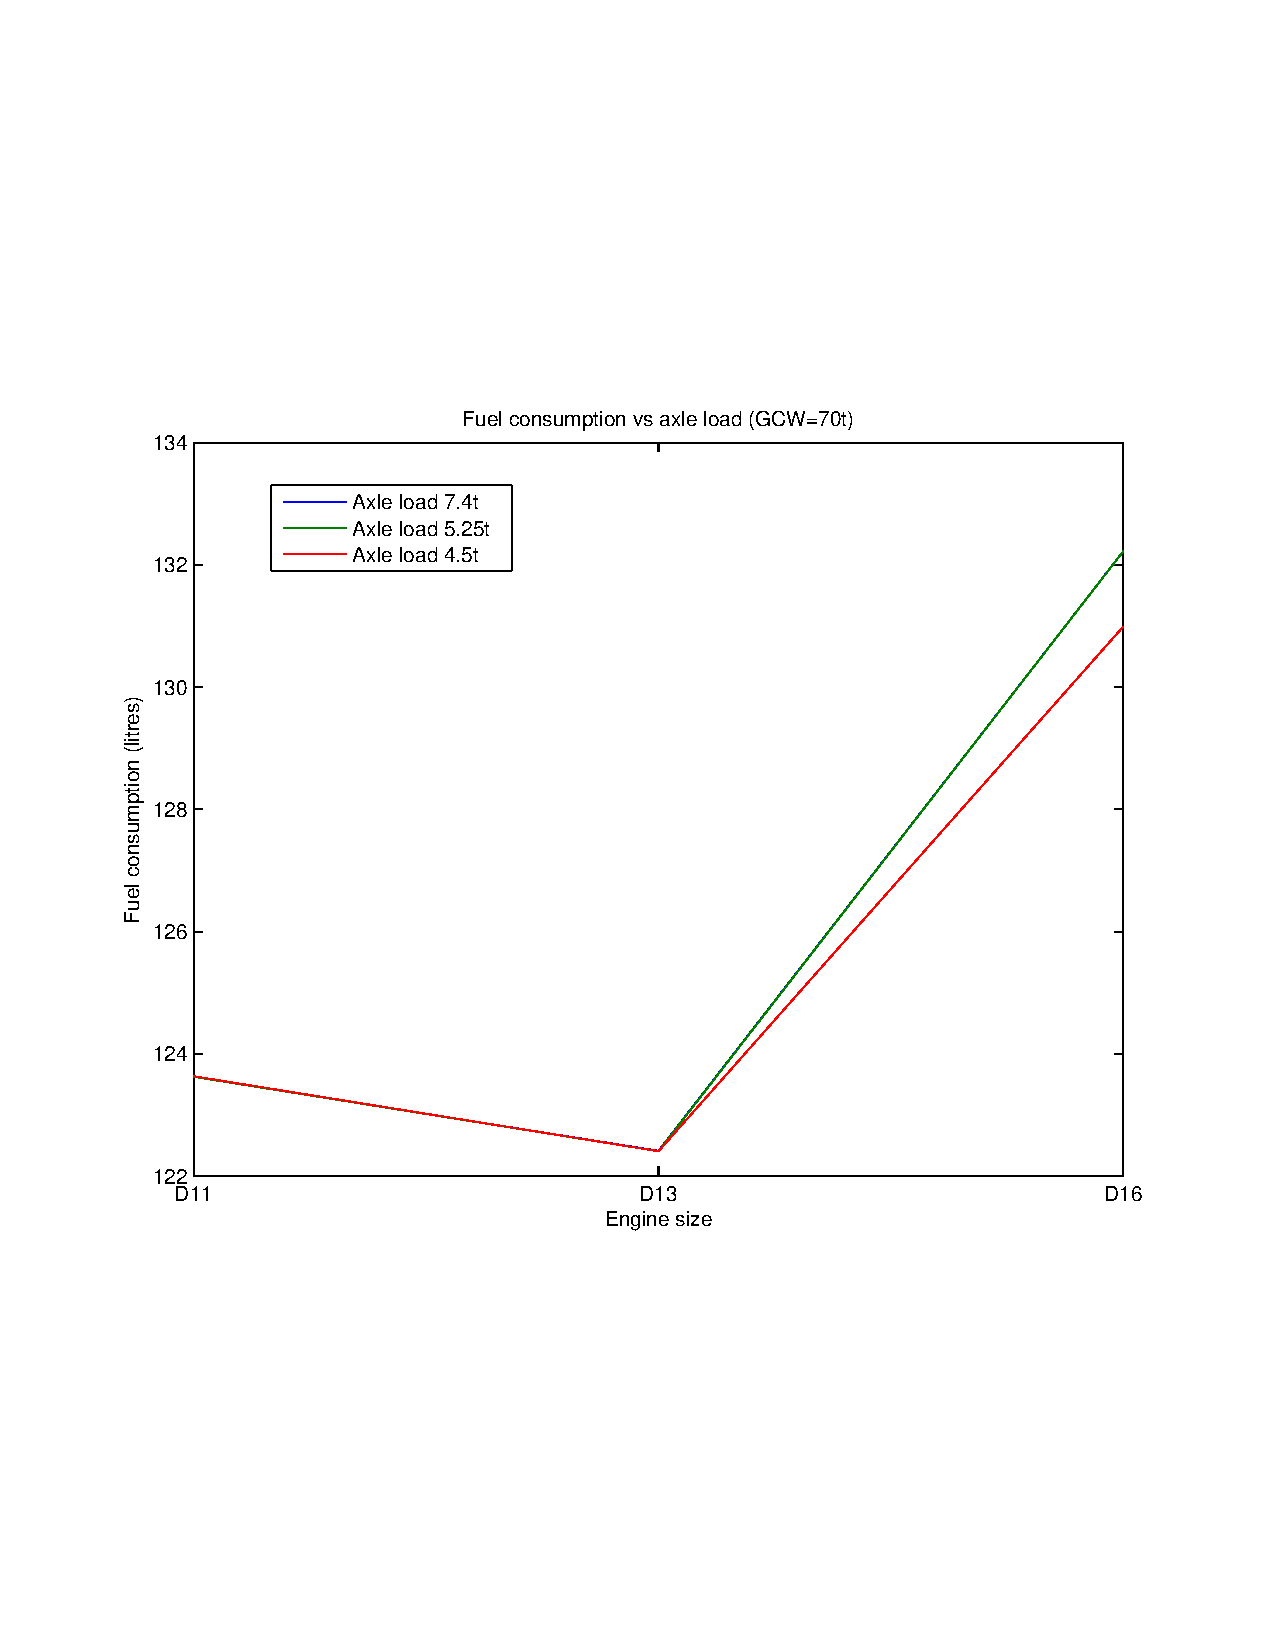
\includegraphics[width=\linewidth, clip=true, trim=45 185 65 206]{figures/ModelValidation/Effect_of_axle_load/Fuel_consumption_vs_axle_load_and_engine_size.pdf}
	\caption{Fuel consumption over mission}
\end{subfigure}
\begin{subfigure}{.5\textwidth}
	\centering
	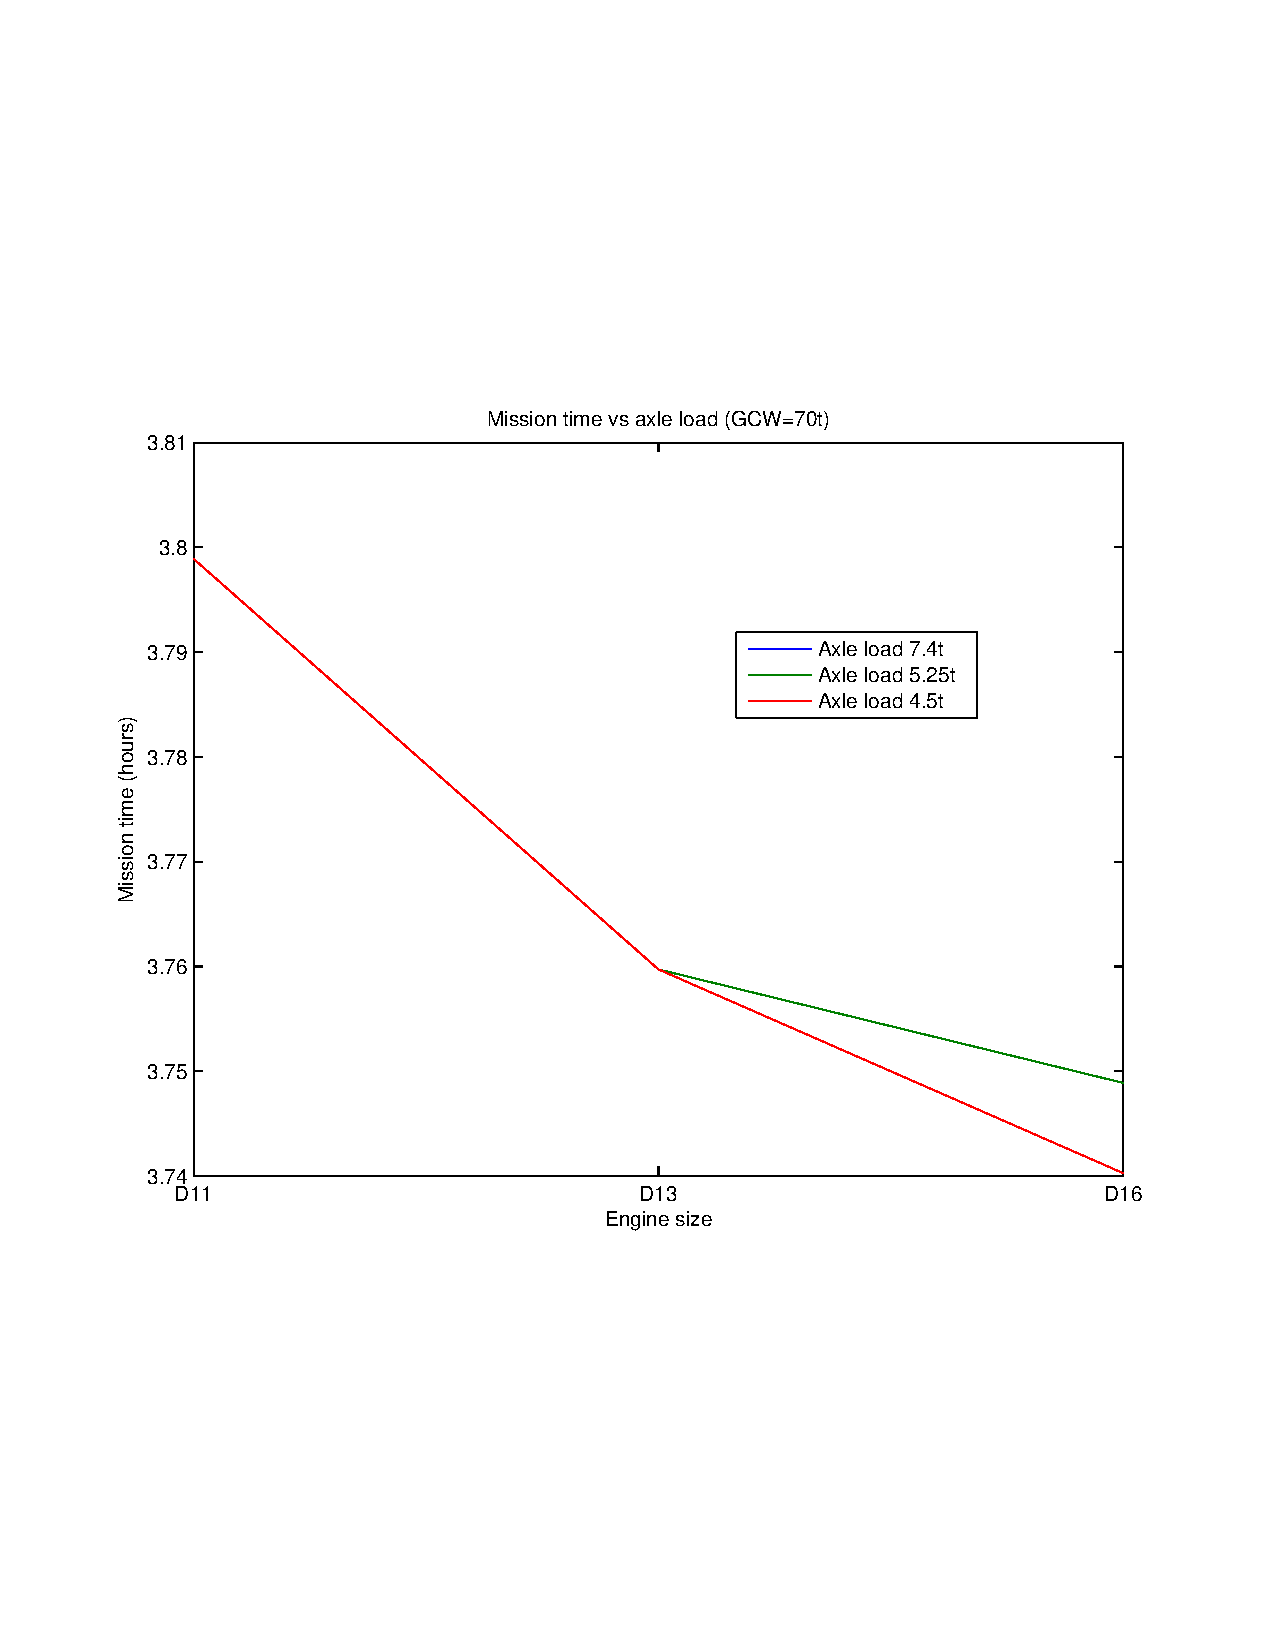
\includegraphics[width=\linewidth, clip=true, trim=45 185 65 206]{figures/ModelValidation/Effect_of_axle_load/Mission_time_vs_axle_load_and_engine_size.pdf}
	\caption{Mission time}
\end{subfigure}
\caption{Effect of axle load on fuel consumption and mission time}
\label{fuelTimeEngineAxleLoad}
\end{figure}

The seemingly curious unchanged fuel consumption and mission times across axle loads for the D11 and D13 engines can be explained by analysing the axle loads in conjunction with power limited operation mode. In the D11 and D13 combinations, even in cases when the tractive force demand was limited by the friction limits of the tire and road, the required power more often than not exceeded the maximum power that the engine and motors could independently produce. This can be seen by comparing the percentage of the mission that the combination was traction limited (as shown in Table \ref{table:tractionLimitMode}) to that when the combination was power limited (as shown in Table \ref{table:powerLimitMode}). In the case of the D16 combinations, when electric propulsion is added to the axle carrying the least load (4.5t), the tractive force demand being grip limited results in the combination being power limited for a smaller fraction of the mission allowing the engine to operate at its optimum point thereby leading to a smaller fuel consumption. The total charge consumption over the mission in each of the cases in shown in Figure \ref{chargeEngineSizeAxleLoad}.\\

\begin{figure}[h!]
\centering
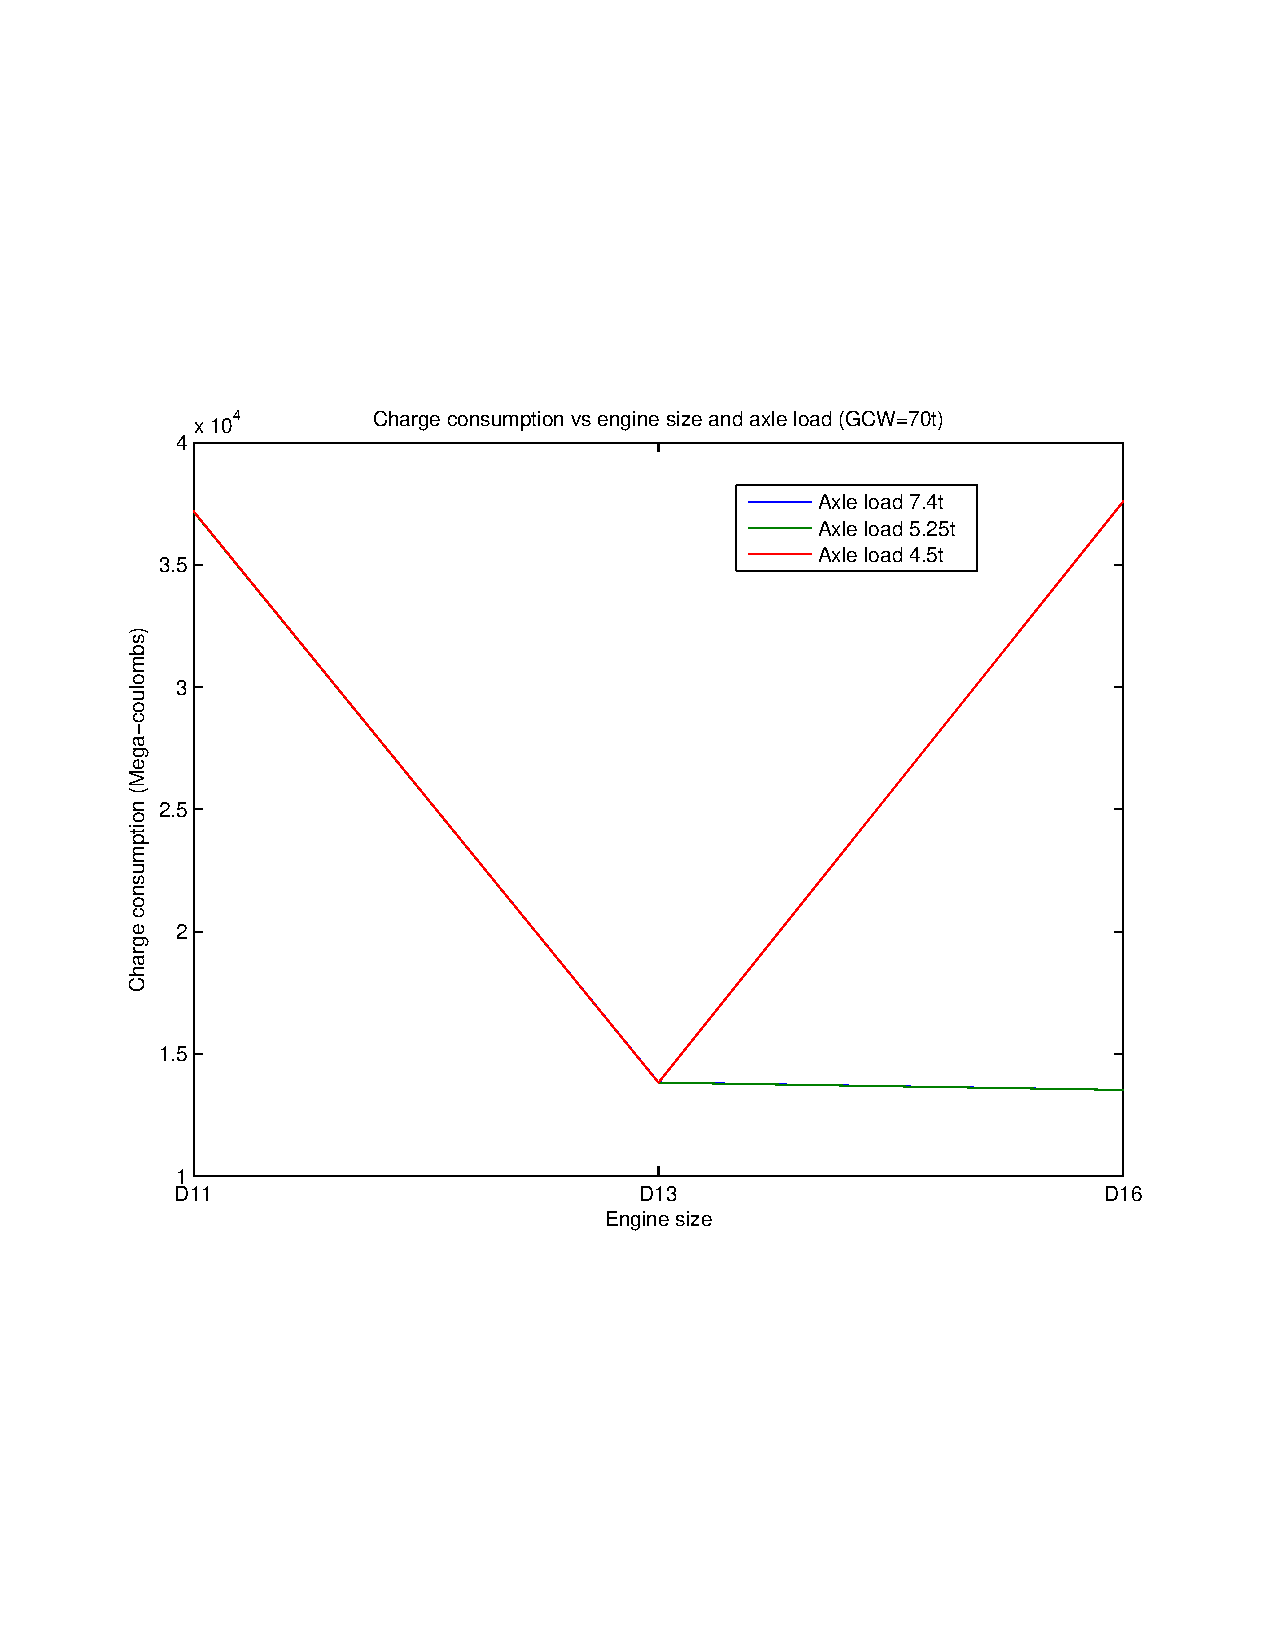
\includegraphics[width=0.5\linewidth, clip=true, trim=45 185 65 208]{figures/ModelValidation/Effect_of_axle_load/Charge_consumption_vs_axle_number_and_axle_load.pdf}
\caption{Effect of engine size and axle load on charge consumption}
\label{chargeEngineSizeAxleLoad}
\end{figure}

\begin{table}[h!]                                       
\centering                                              
\begin{tabular}{|c|c|c|c|}                              
\hline                                                  
 & Axle Load 7.4t & Axle Load 5.25t & Axle Load 4.5t \\
 & 011-010-00-000 & 011-000-01-000 & 011-000-00-010 \\
\hline                                                  
D11 & 5.31 & 5.63 & 5.75 \\                            
\hline                                                  
D13 & 3.01 & 3.13 & 3.17 \\ 
\hline                              
D16 & 2.10 & 2.18 & 1.79 \\                                
\hline                                                  
\end{tabular}                                           
\caption{Percentage of the mission that was traction-limited}                                
\label{table:tractionLimitMode}                              
\end{table}  

\begin{table}[h!]                                       
\centering                                              
\begin{tabular}{|c|c|c|c|}                              
\hline                                                  
 & Axle Load 7.4t & Axle Load 5.25t & Axle Load 4.5t \\
 & 011-010-00-000 & 011-000-01-000 & 011-000-00-010 \\
\hline                                                  
D11 & 10.85 & 10.85 & 10.84 \\                            
\hline                                                  
D13 & 5.64 & 5.64 & 5.64 \\ 
\hline                              
D16 & 5.53 & 5.53 & 4.34 \\                                
\hline                                                  
\end{tabular}                                           
\caption{Percentage of the mission operating in power-limit mode}                                
\label{table:powerLimitMode}                              
\end{table}  

The startability of the combinations can thus be analysed in a similar manner and is depicted in Figure \ref{startabilityEngineAxleLoad}.\\

\begin{figure}[h!]
\centering
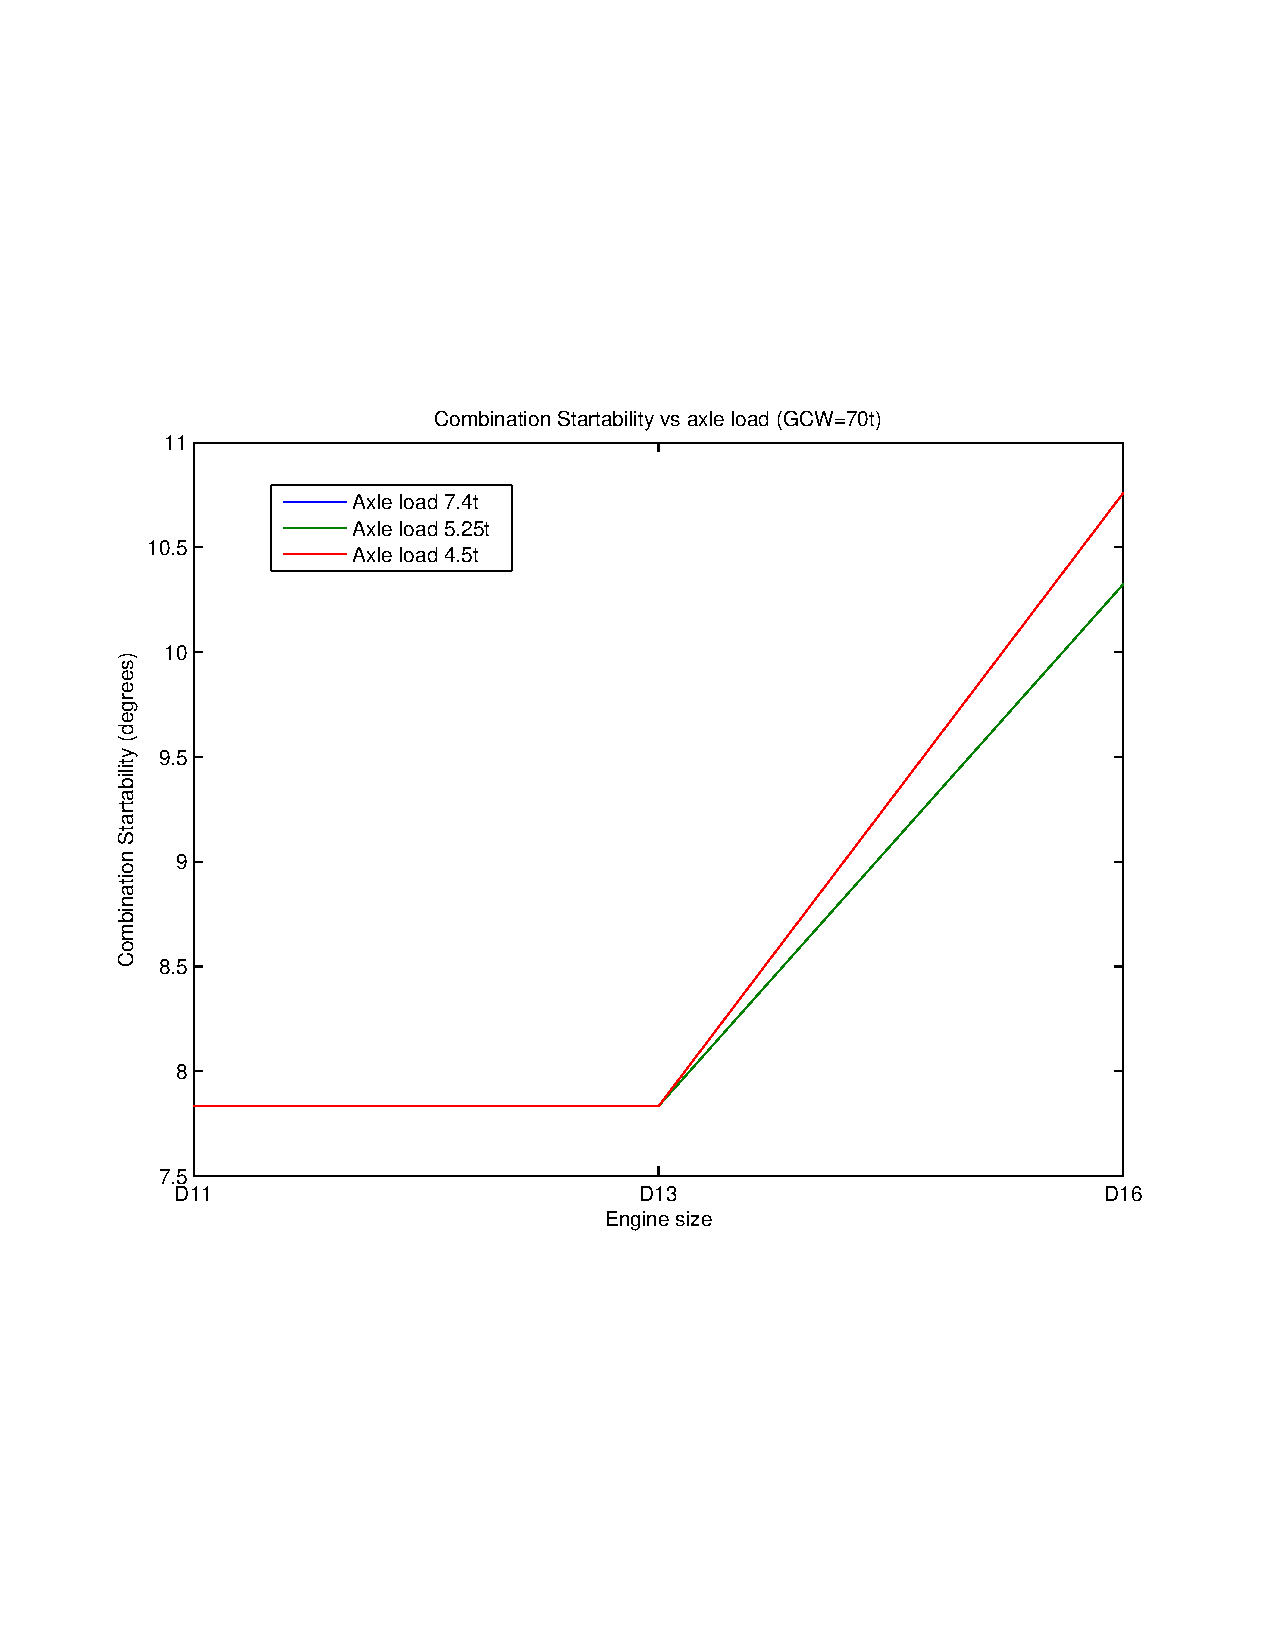
\includegraphics[width=0.5\linewidth, clip=true, trim=45 185 65 208]{figures/ModelValidation/Effect_of_axle_load/Combination_startability_vs_axle_load_and_engine_size.pdf}
\caption{Effect of engine size and axle load on combination startability}
\label{startabilityEngineAxleLoad}
\end{figure}

\subsection{Machine power / torque rating}

Combined with the axle load problem is one of choosing the right electric machine rating for the axle. The effect of the machine rating is direct in that the torque available at the axle is varied by the choice of the rating. The D13 engine powered 011-010-00-000 combination with a GCW of 70t is chosen for this exercise. The combination is simulated with varying electric machine ratings. The fuel consumption and mission time in each of the cases is depicted in Figure \ref{fuelTimeEngineAxleLoad}.\\

\begin{figure}[h!]
\begin{subfigure}{.5\textwidth}
	\centering
	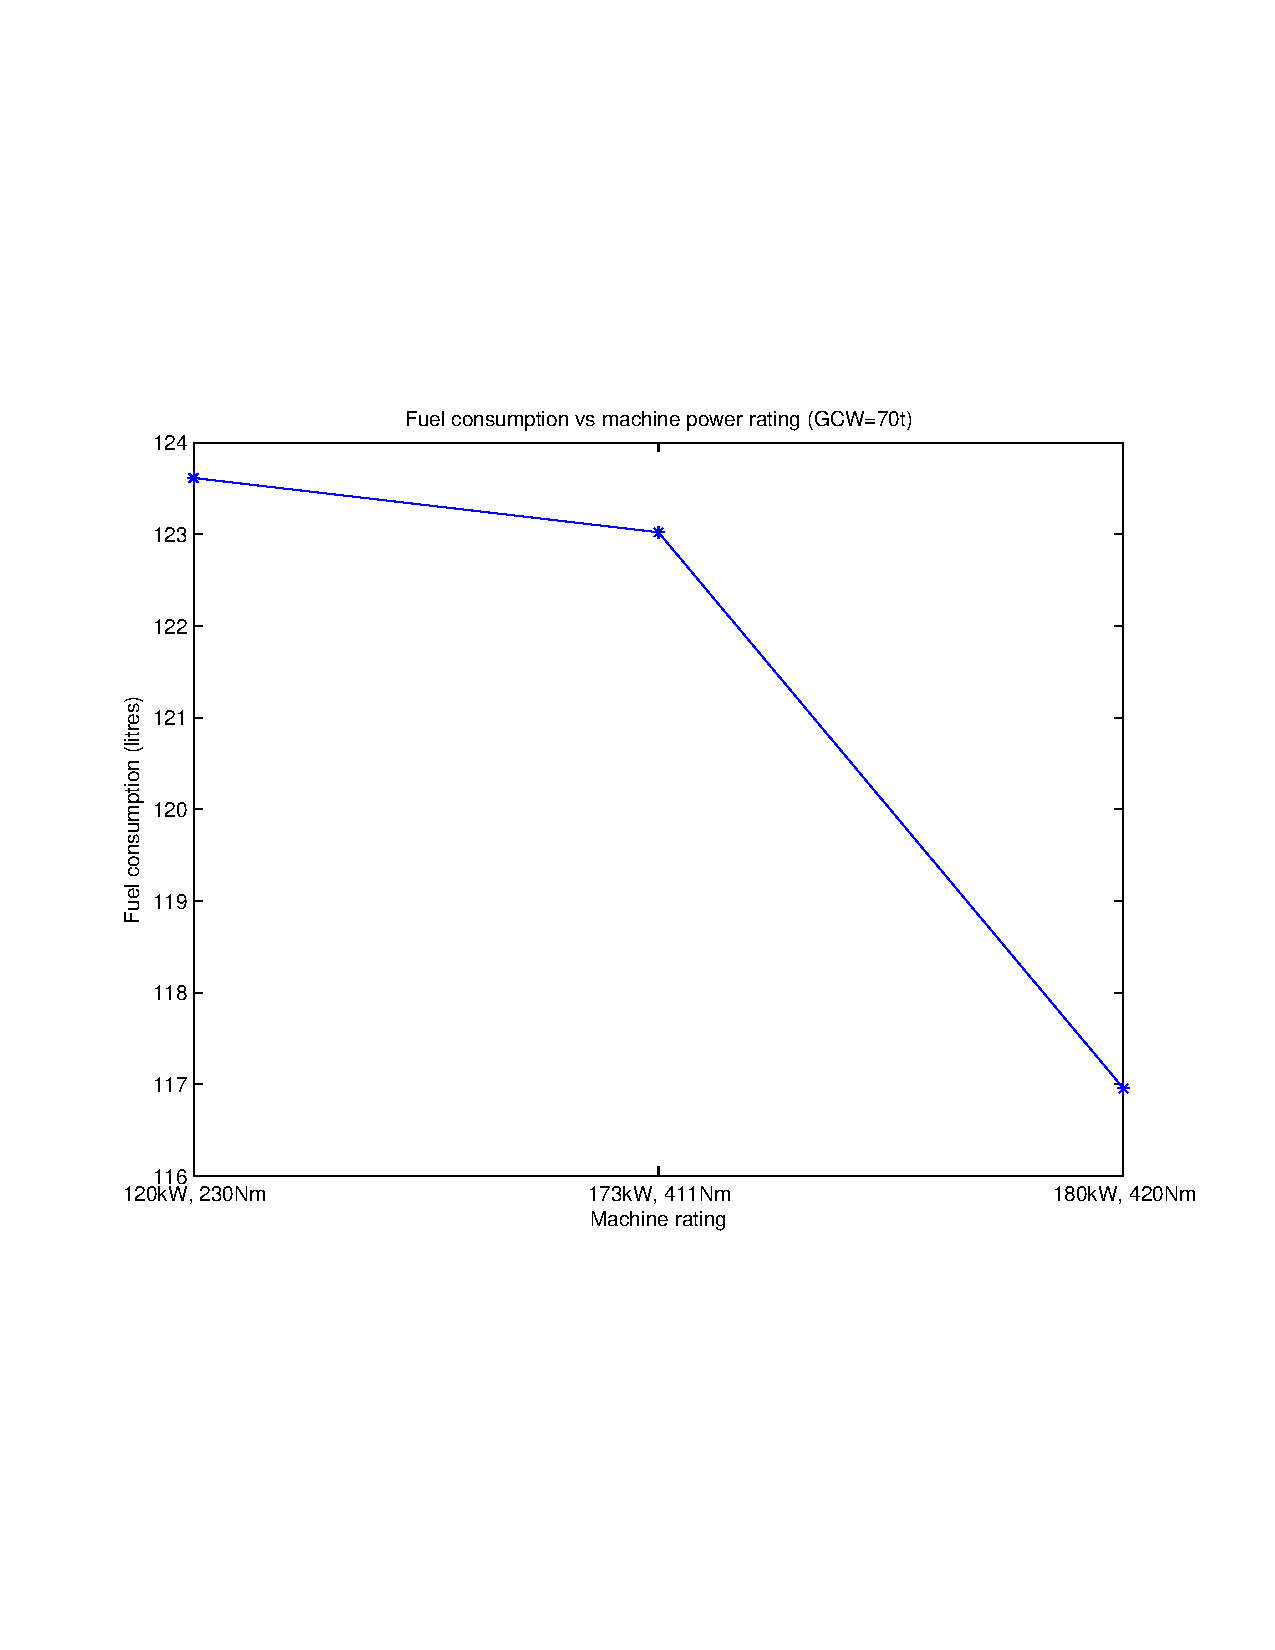
\includegraphics[width=\linewidth, clip=true, trim=45 185 65 206]{figures/ModelValidation/Effect_of_machine_power_rating/Fuel_consumption_vs_machine_power_rating.pdf}
	\caption{Fuel consumption over mission}
\end{subfigure}
\begin{subfigure}{.5\textwidth}
	\centering
	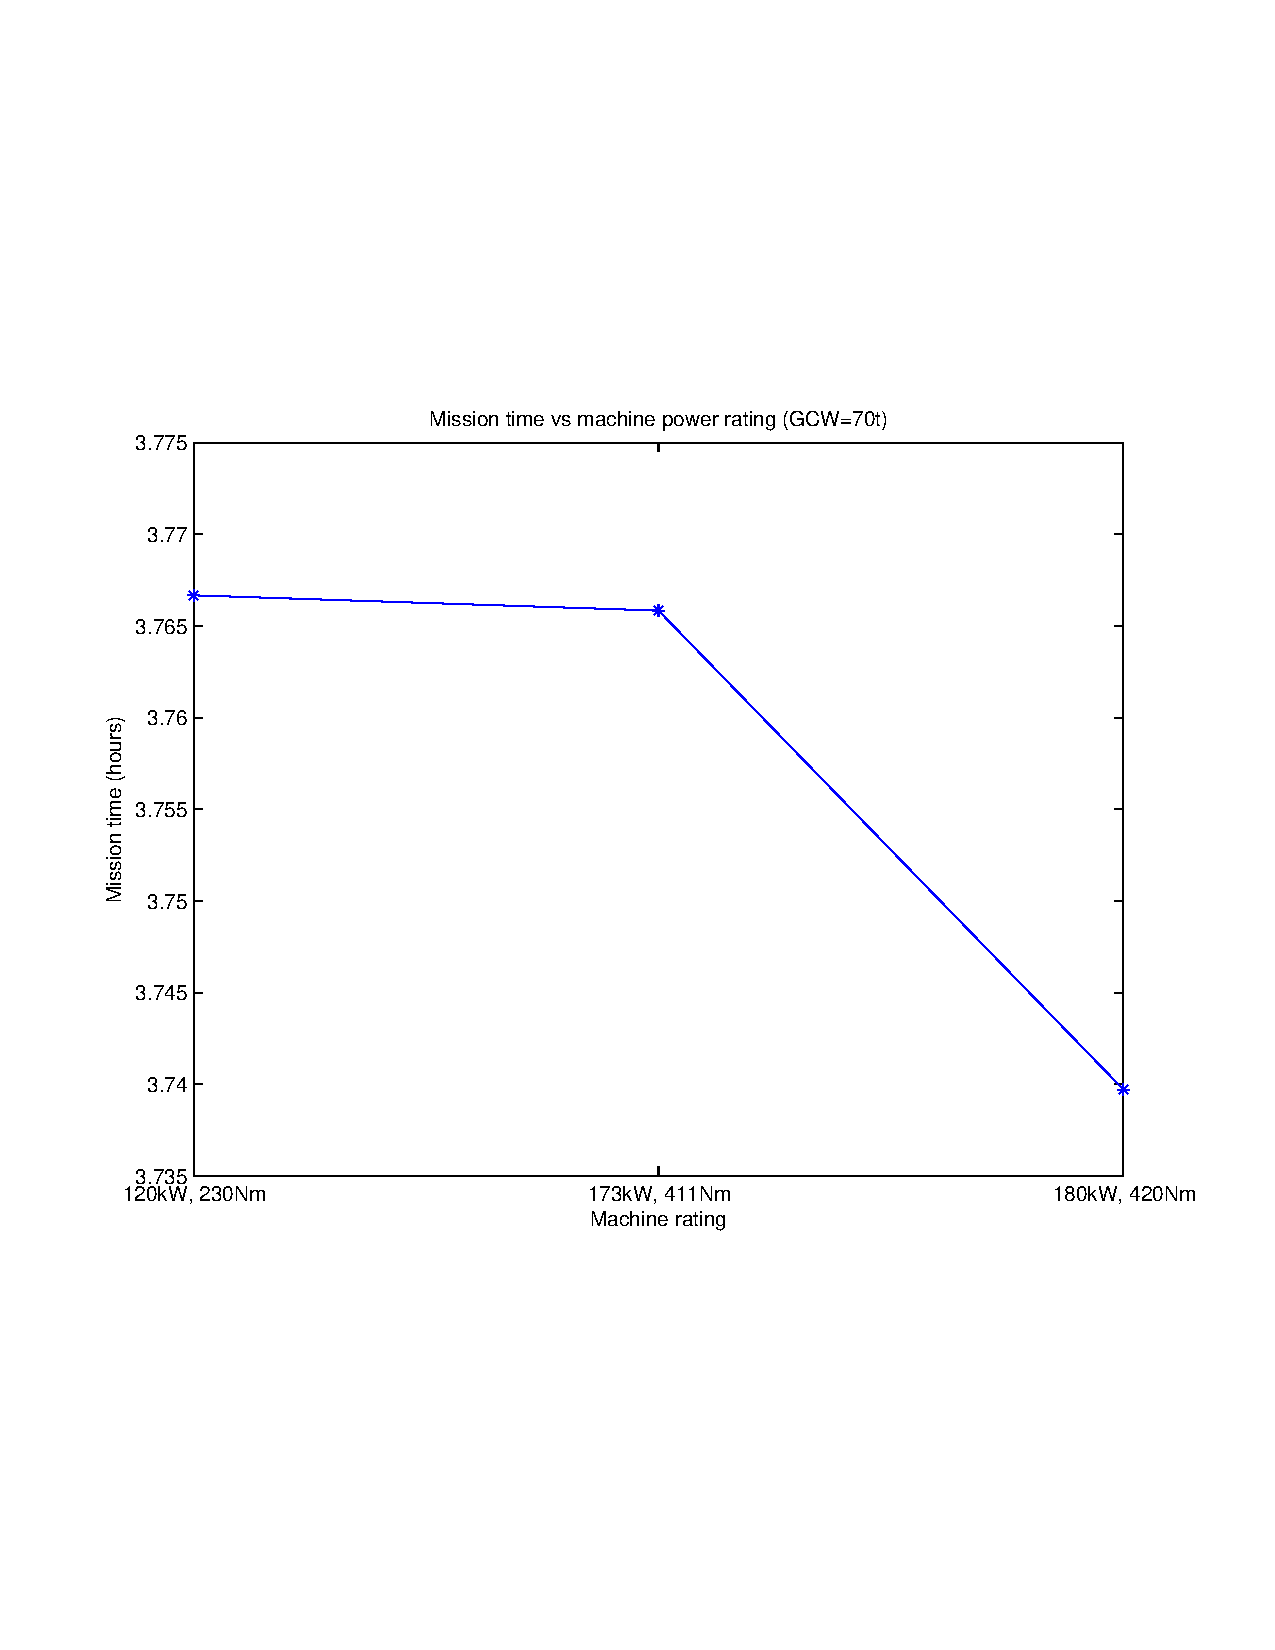
\includegraphics[width=\linewidth, clip=true, trim=45 185 65 206]{figures/ModelValidation/Effect_of_machine_power_rating/Mission_time_vs_machine_power_rating.pdf}
	\caption{Mission time}
\end{subfigure}
\caption{Effect of machine power rating on fuel consumption and mission time}
\label{fuelTimeEngineAxleLoad}
\end{figure}

The reduction in fuel consumption arising from additionally available electric propulsion is clearly seen in Figure \ref{fuelTimeEngineAxleLoad}. A fuel saving of 5.4\% is obtained from using the 180kW, 420Nm motor in place of the 120kW, 230Nm one. Also, the combination speed at the peak of Hallands\aa sen is improved by close to 2.5ms\textsuperscript{-1} from 8.59ms\textsuperscript{-1} to 11.05ms\textsuperscript{-1} as can be seen in Figure \ref{speedMissionMachineRating}.\\

\begin{figure}[h!]
\centering
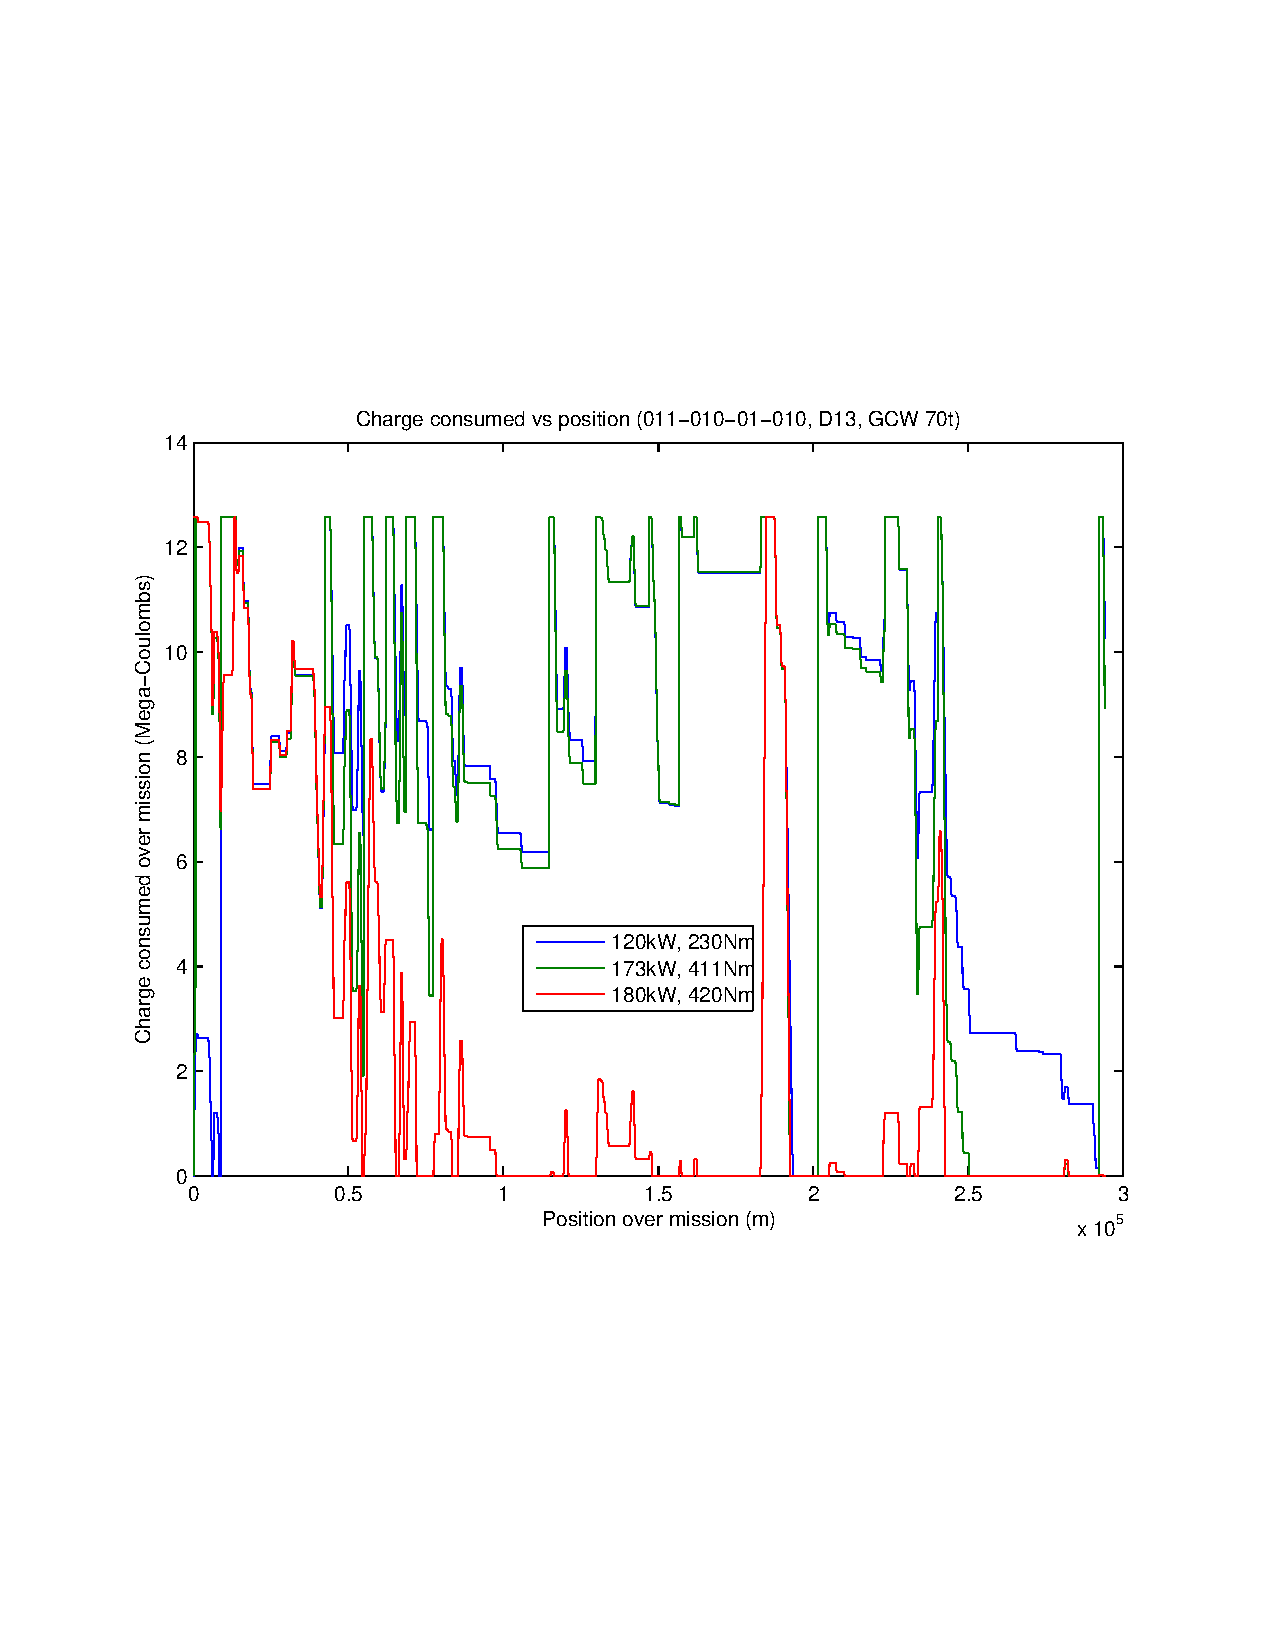
\includegraphics[width=\linewidth, clip=true, trim=45 185 65 208]{figures/ModelValidation/Effect_of_machine_power_rating/Charge_consumed_vs_position_(011-010-01-010,D13,GCW_70t).pdf}
\caption{Effect of machine power rating on charge consumption over mission}
\label{chargeMissionMachineRating}
\end{figure}

\begin{figure}[h!]
\centering
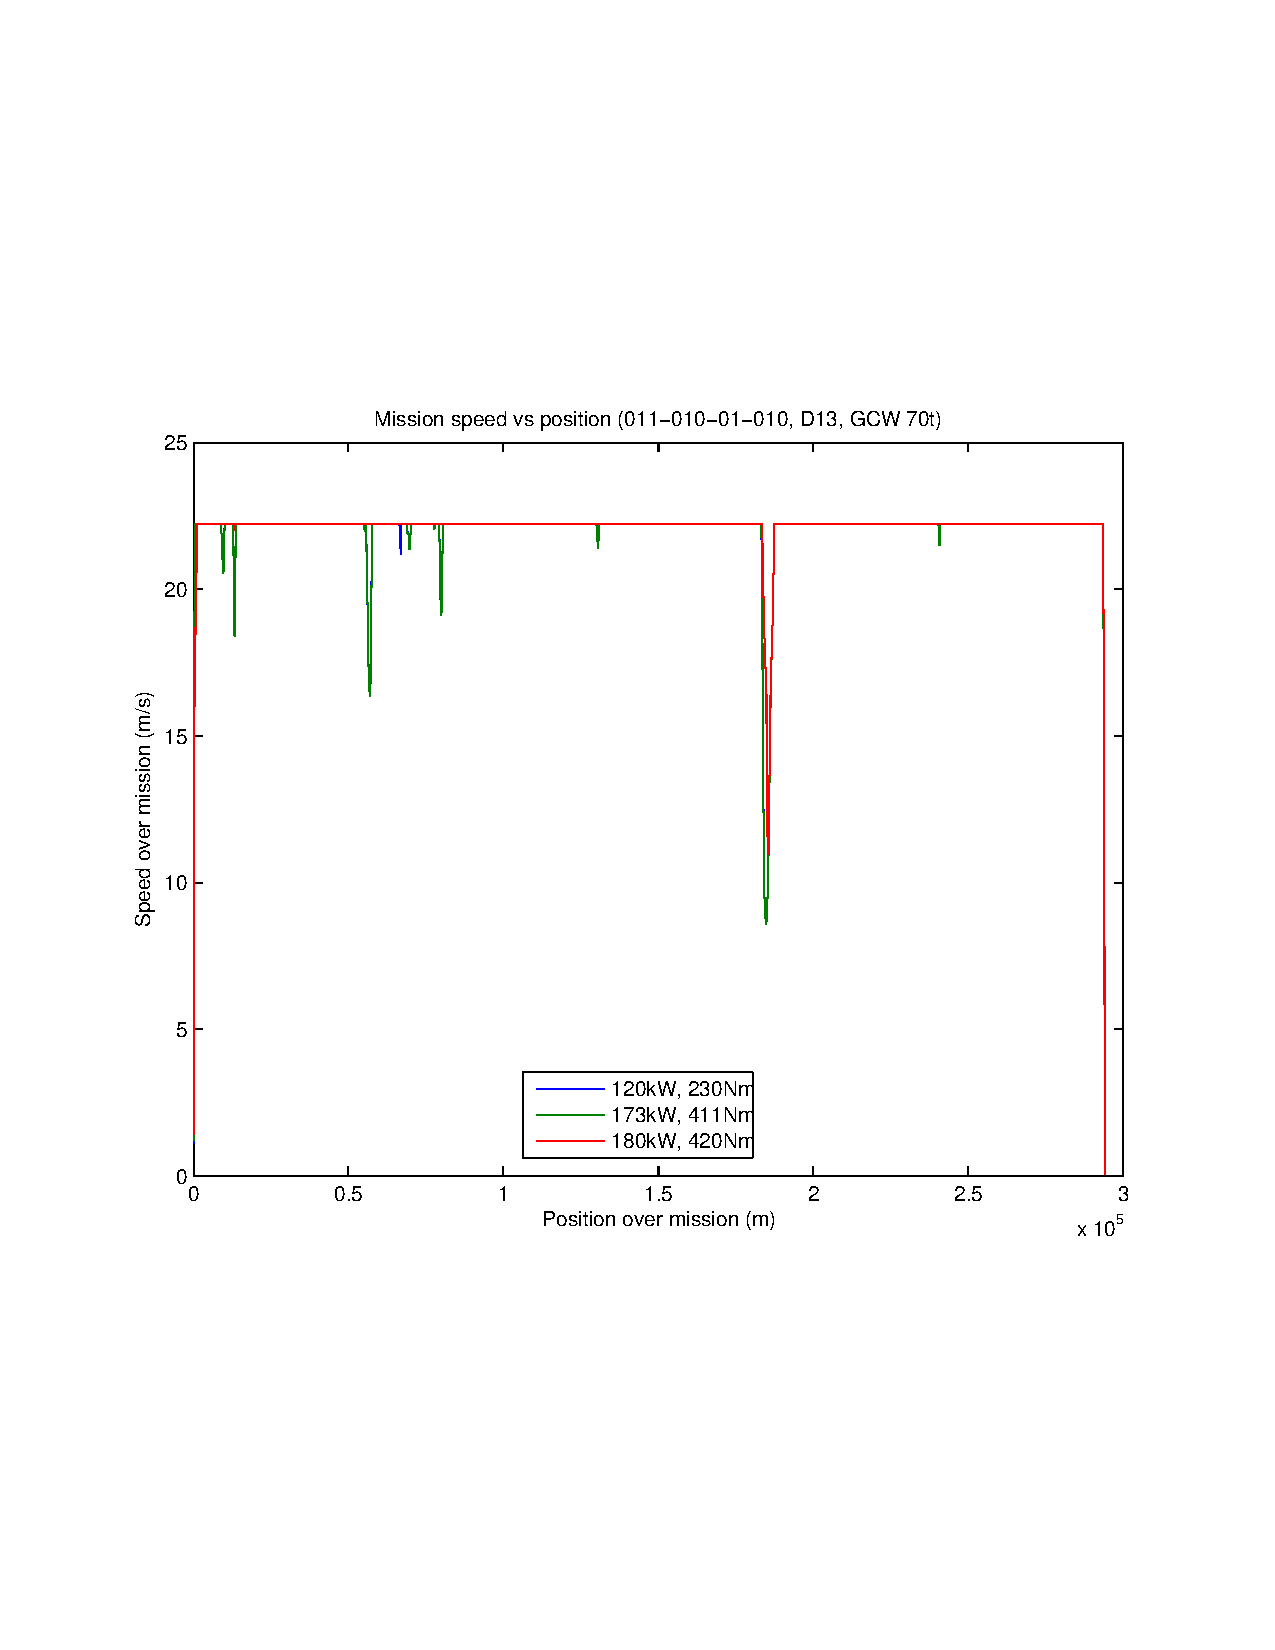
\includegraphics[width=\linewidth, clip=true, trim=45 185 65 208]{figures/ModelValidation/Effect_of_machine_power_rating/Mission_speed_vs_position_(011-010-01-010,D13,GCW_70t).pdf}
\caption{Effect of machine power rating on vehicle speed over mission}
\label{speedMissionMachineRating}
\end{figure}

The choice of the machine rating is of course beset with the heavier costs associated with the machine and its auxiliaries. The productivity of the mission hence includes both these factors. Also, the reduced payload carrying capacity that results from higher rated machines being heavier is also factored while calculating mission revenues for mission productivity.\\

\subsection{Engine downsizing}

The effect of downsizing the combustion engine on combinations with electrically propelled trailer axles is key to reducing mission costs and improving fuel economy thereby doubling boosting mission productivity. The 011-010-01-010 combination with a GCW of 70t is chosen and the combustion engine size is varied to observe the trends in fue consumption and mission time among other combination parameters.\\

\begin{figure}[h!]
\begin{subfigure}{.5\textwidth}
	\centering
	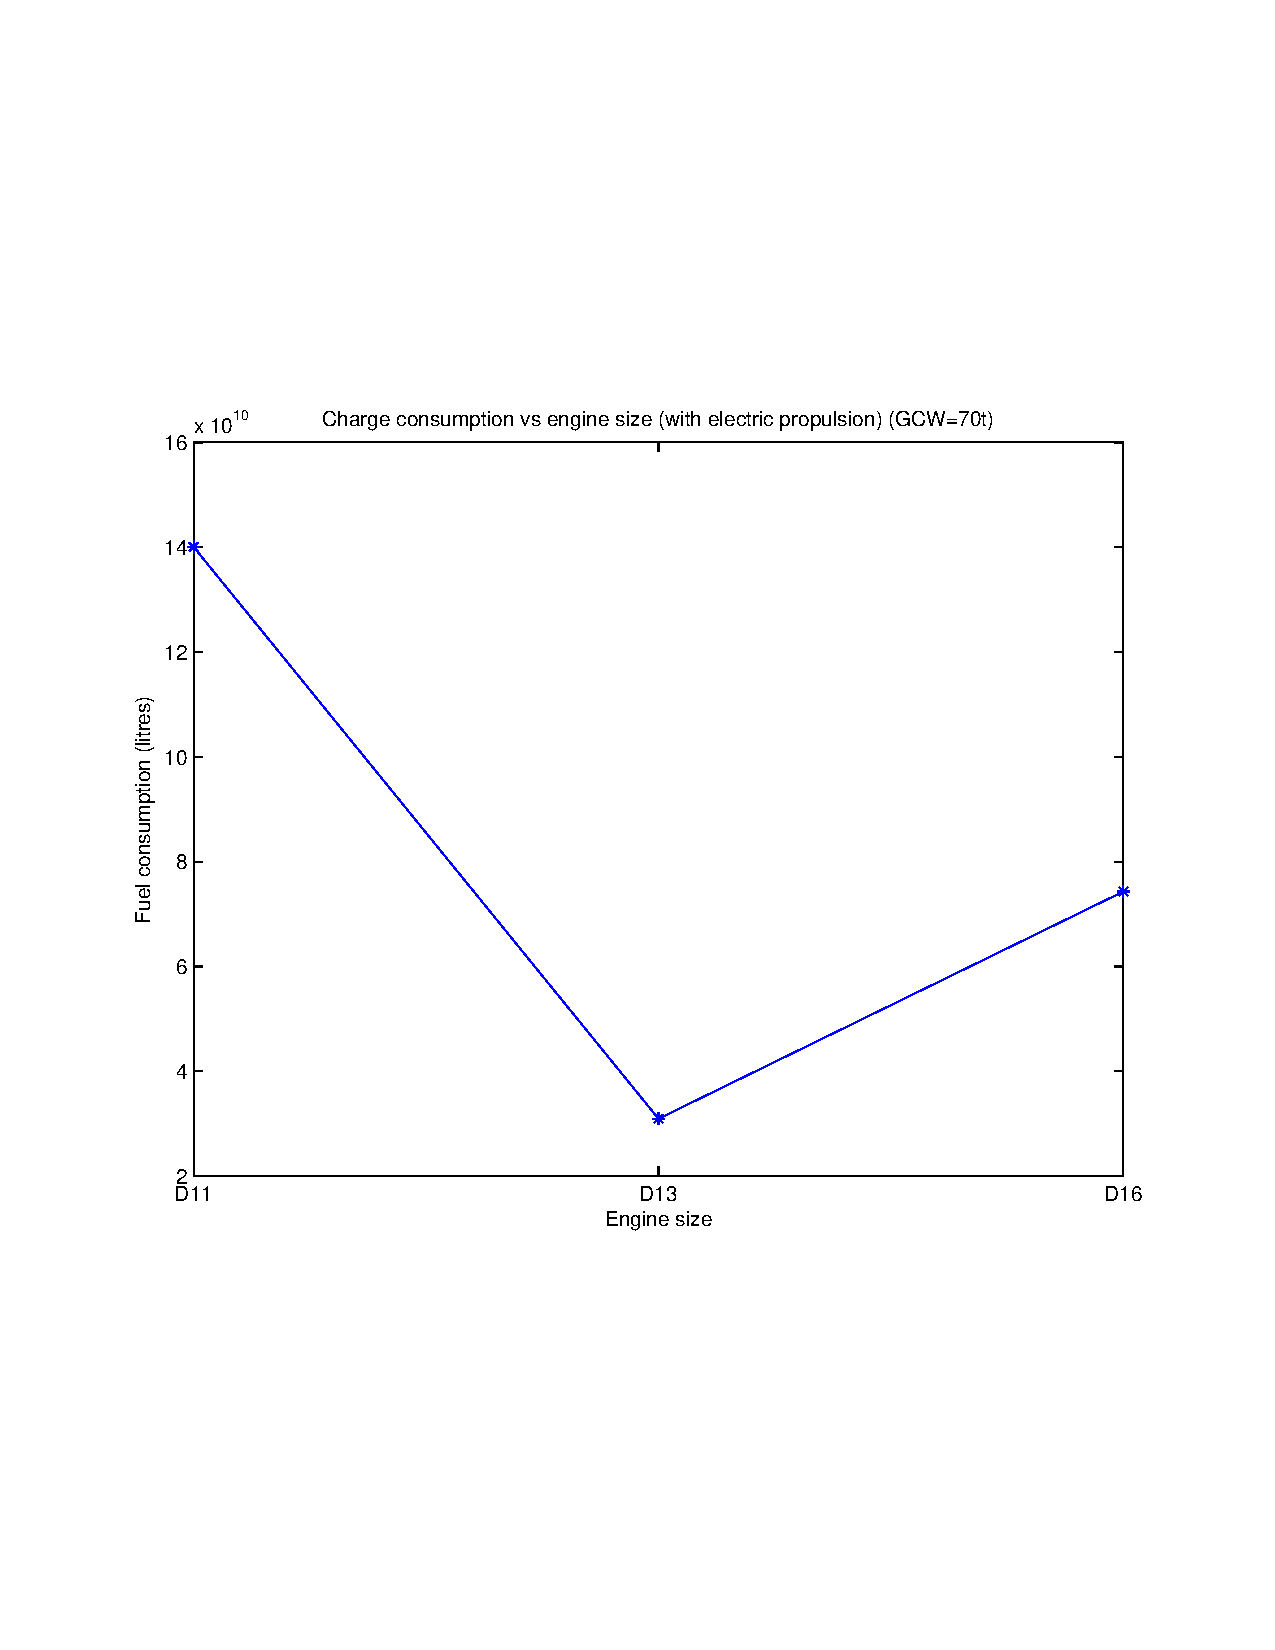
\includegraphics[width=\linewidth, clip=true, trim=45 185 65 206]{figures/ModelValidation/Engine_downsizing/Fuel_consumption_vs_engine_size_(with_electric_propulsion).pdf}
	\caption{Fuel consumption over mission}
\end{subfigure}
\begin{subfigure}{.5\textwidth}
	\centering
	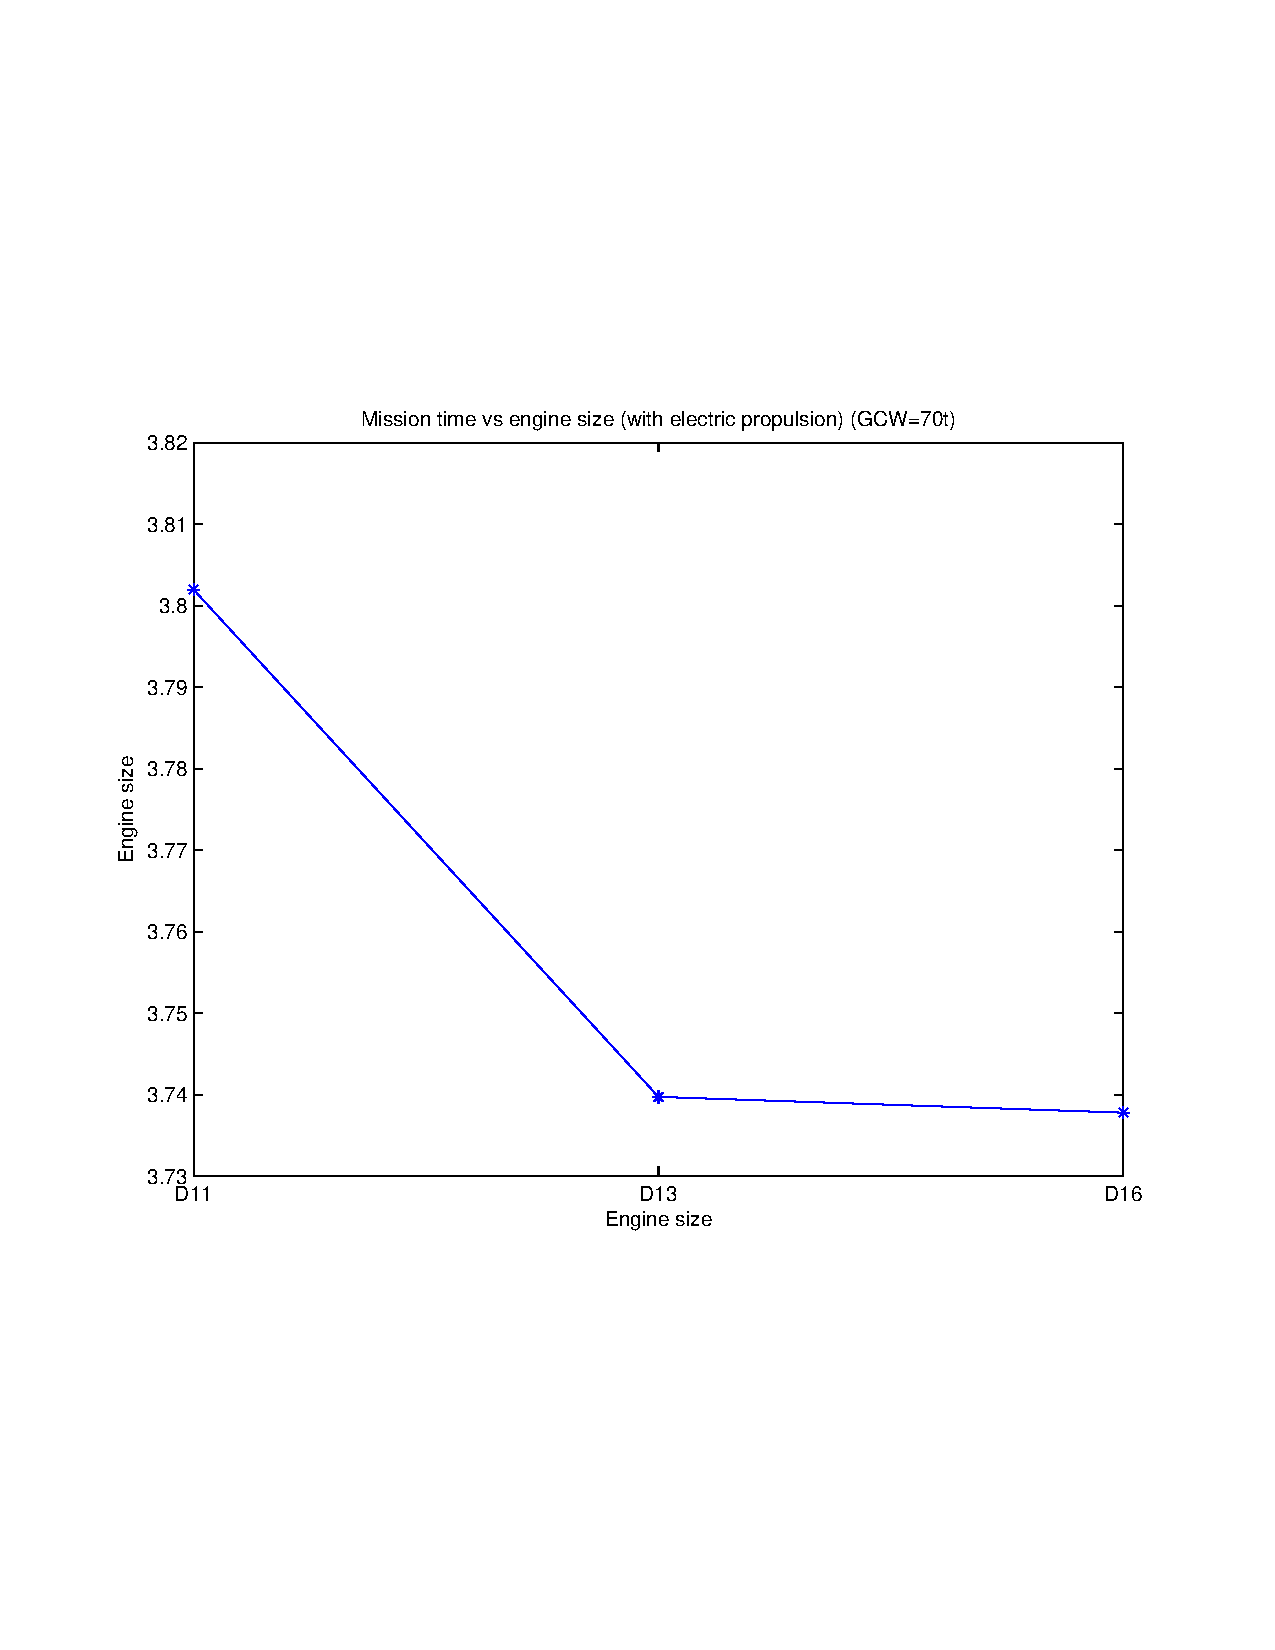
\includegraphics[width=\linewidth, clip=true, trim=45 185 65 206]{figures/ModelValidation/Engine_downsizing/Mission_time_vs_engine_size_(with_electric_propulsion)(GCW=70t).pdf}
	\caption{Mission time}
\end{subfigure}
\caption{Effect of engine downsizing on fuel consumption and mission time}
\label{fuelTimeEngineDownsize}
\end{figure}

\begin{figure}[h!]
\centering
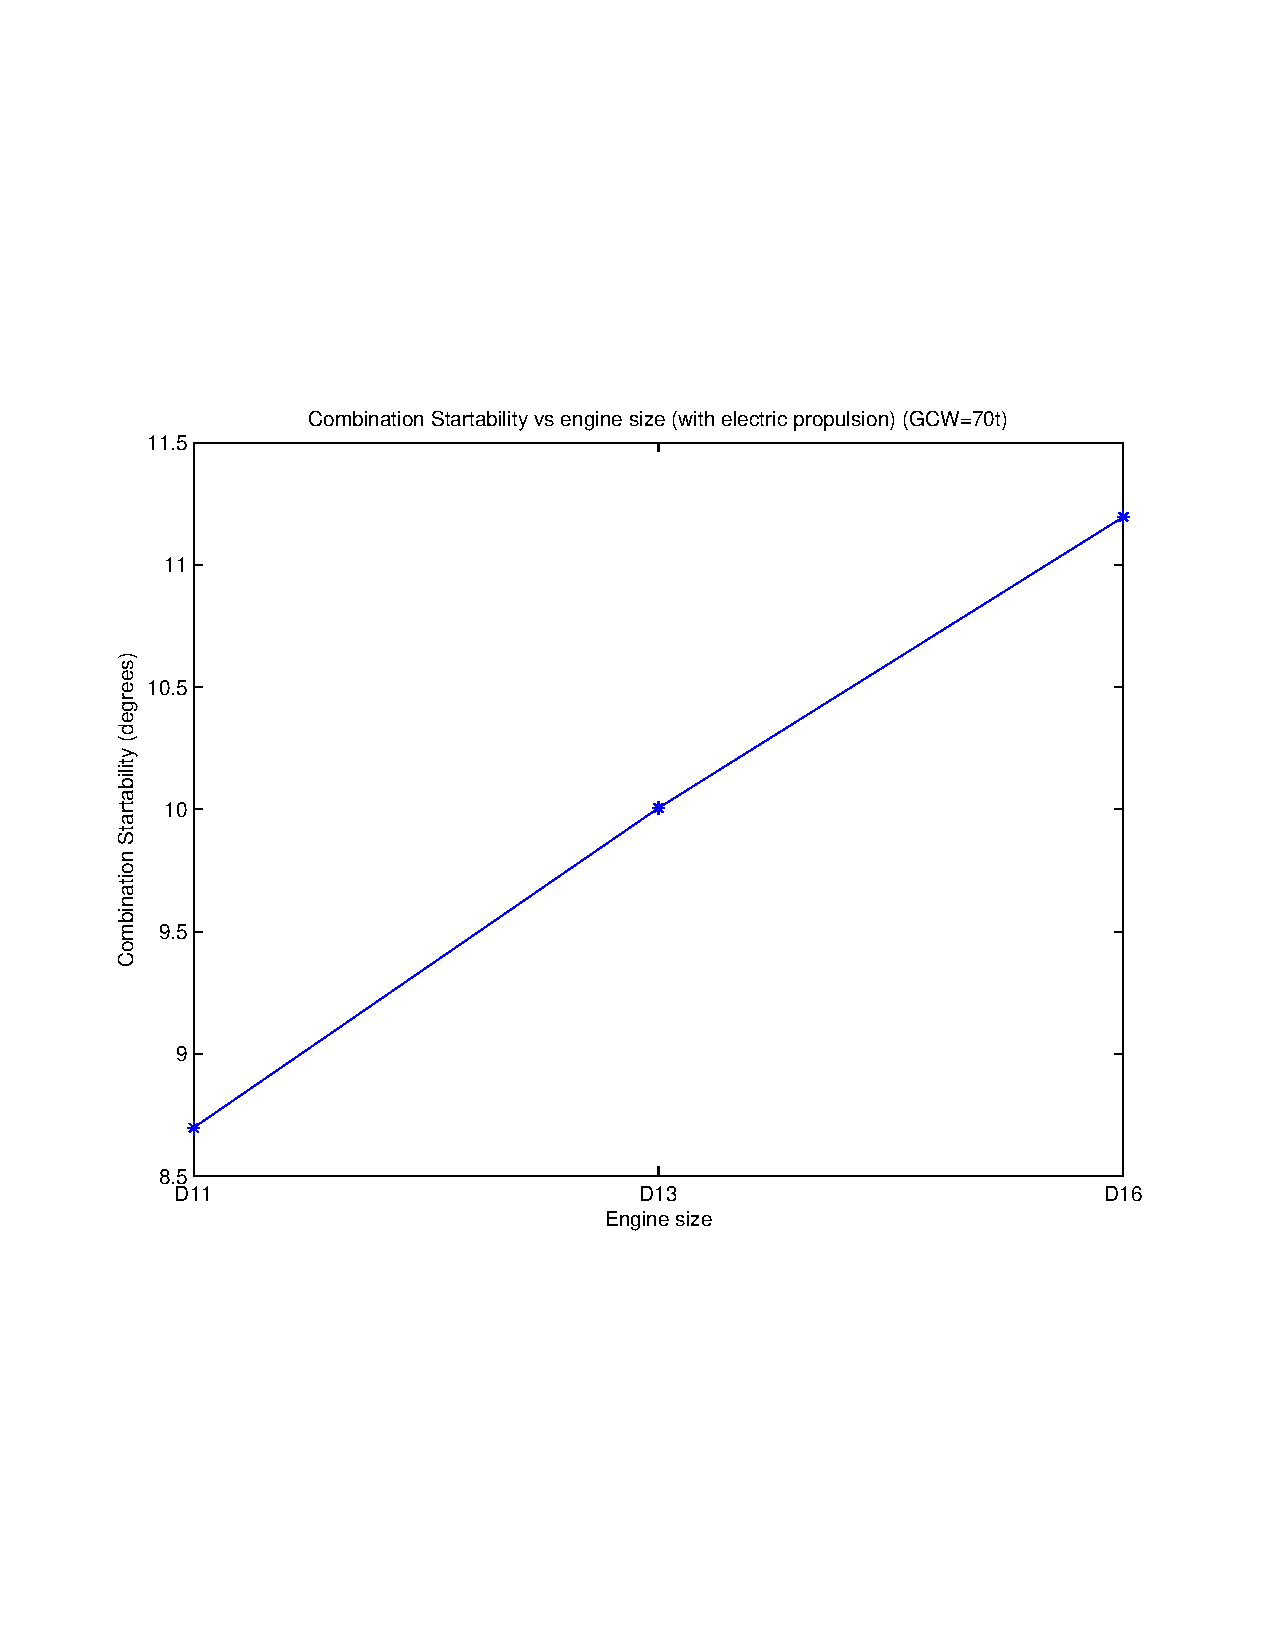
\includegraphics[width=0.5\linewidth, clip=true, trim=45 185 65 208]{figures/ModelValidation/Engine_downsizing/Combination_startability_vs_engine_size_(with_electric_propulsion).pdf}
\caption{Effect of engine downsizing on combination startability}
\label{startabilityEngineDownsize}
\end{figure}

The benefits of choosing the D13 engine over the D16 engine merely based on the fuel economy and comparable mission time is evident, as can be seen in Figure \ref{fuelTimeEngineDownsize}. As expected, the startability of the 70t combination is advantaged by increasing engine size and is shown in Figure \ref{startabilityEngineDownsize}. It must be noted that since the mission times are comparable in case of the D13 and D16 engines, the advantage gained through increased gradeability over Hallands\aa sen and improved average speeds is inconsequential over the mission. The improved fuel economy for the given mission can also be traced to the fact that the percentage of the mission that is power limited in both cases (D13 and D16)  is similar at 2.47\% and 3.9\% respectively.\\

This observation is significant as it justifies the use of smaller engines combined with additional electric propulsion in order to be able to utilise gradient-derived potential energy more efficiently in place of fuel-derived energy. The case for choosing smaller engines owing to them being less expensive and lighter is also thus motivated.\\

As expected, the drop in vehicle speed at gradients is more significant in the case of the smaller engine as can be seen in Figure \ref{speedEngineDownsizing}.\\

\begin{figure}[h!]
\centering
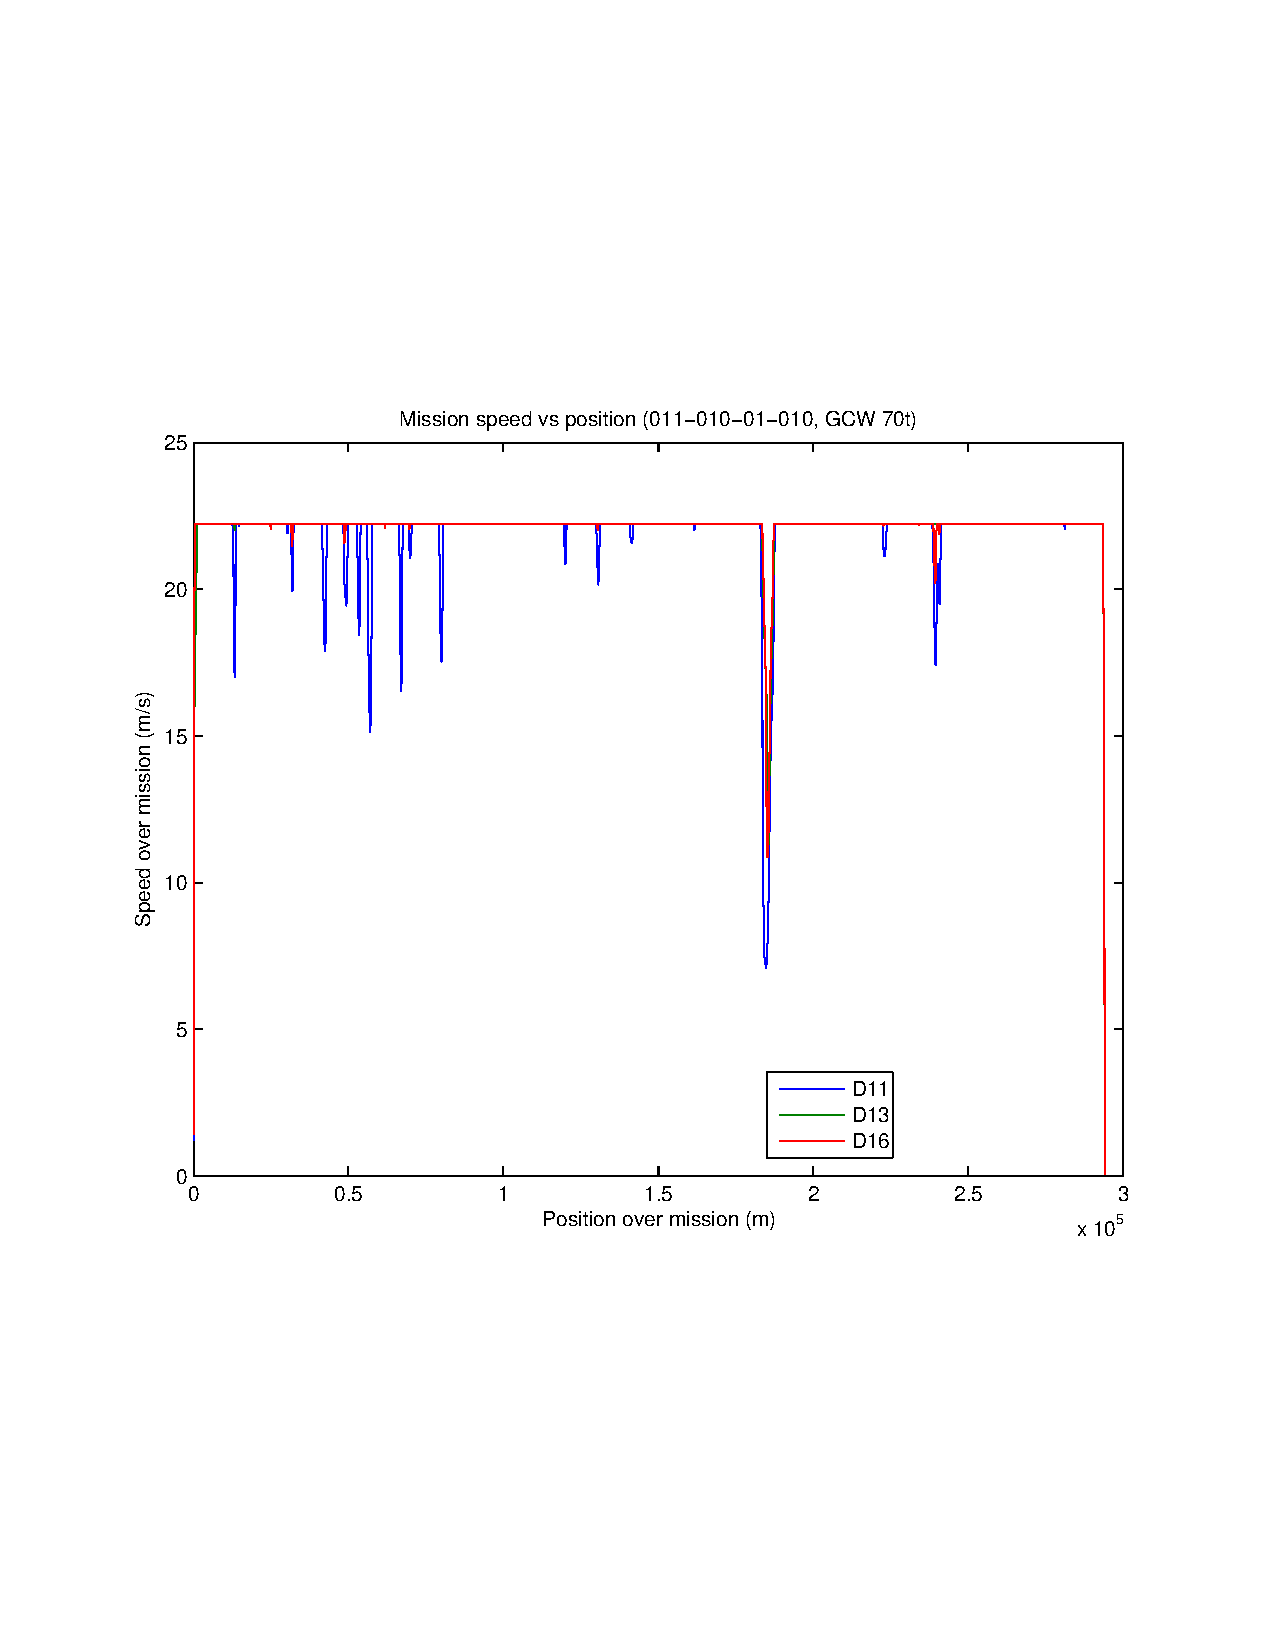
\includegraphics[width=0.8\linewidth, clip=true, trim=45 185 65 208]{figures/ModelValidation/Engine_downsizing/Mission_speed_vs_position_(011-010-01-010,GCW_70t).pdf}
\caption{Effect of engine downsizing on vehicle speed over mission}
\label{speedEngineDownsizing}
\end{figure}

\subsection{Buffer Size}

The choice of buffer size dictates the availability of electric power over the mission and also determines the regeneration potential of the vehicle. Three electric buffers of sizes 4976640, 6272640 and 5987500 Coulombs were used to study the same. These are derived from Volvo's list of available energy buffers as of date.



\end{document}